\documentclass[hess, manuscript]{copernicus}
%DIF LATEXDIFF DIFFERENCE FILE
%DIF DEL ../v1_1_preprint/main.tex   Wed Jun 10 10:27:29 2026
%DIF ADD main.tex                    Tue Jun 30 22:34:14 2026

% --- Encodage, langue, fontes ---
%DIF 4-8d4
%DIF < \ifPDFTeX
%DIF <   \usepackage[english]{babel}
%DIF < \else
%DIF <   \babelprovide[main,import]{english}
%DIF < \fi
%DIF -------

% --- Mise en page, microtypographie ---
% \usepackage[margin=1.5cm]{geometry}
\usepackage{microtype}
\setlength{\parindent}{0pt}
\setlength{\parskip}{6pt}
\usepackage{ragged2e}
\usepackage[percent]{overpic} % coordonnées en %

% --- Maths ---
\usepackage{amsmath}
\ifPDFTeX
  \usepackage{amssymb}
\fi

% --- Sections non numérotées (style mémo/rapport court) ---
%DIF 25d20
%DIF < %\setcounter{secnumdepth}{3}
%DIF -------

% --- Couleurs, figures, tableaux ---
\usepackage{xcolor}
\usepackage{graphicx}
\usepackage{booktabs,longtable,tabularx,multirow}
\usepackage{float}
\usepackage{caption}
\usepackage{subcaption}

% --- Liens et URLs ---
\usepackage{xurl}
\usepackage{hyperref}

% --- Bibliographie (Style Copernicus) ---
\usepackage[authoryear]{natbib}
\bibliographystyle{copernicus}

% --- Compat Pandoc/Quarto ---
\providecommand{\tightlist}{\setlength{\itemsep}{0pt}\setlength{\parskip}{0pt}}

% --- Numéros de lignes (optionnel) ---
% \usepackage{setspace}
% \doublespacing

% --- DEBUT ---
%DIF PREAMBLE EXTENSION ADDED BY LATEXDIFF
%DIF UNDERLINE PREAMBLE %DIF PREAMBLE
\RequirePackage[normalem]{ulem} %DIF PREAMBLE
\RequirePackage{color}\definecolor{RED}{rgb}{1,0,0}\definecolor{BLUE}{rgb}{0,0,1} %DIF PREAMBLE
\providecommand{\DIFaddtex}[1]{{\protect\color{blue}\uwave{#1}}} %DIF PREAMBLE
\providecommand{\DIFdeltex}[1]{{\protect\color{red}\sout{#1}}} %DIF PREAMBLE
%DIF SAFE PREAMBLE %DIF PREAMBLE
\providecommand{\DIFaddbegin}{} %DIF PREAMBLE
\providecommand{\DIFaddend}{} %DIF PREAMBLE
\providecommand{\DIFdelbegin}{} %DIF PREAMBLE
\providecommand{\DIFdelend}{} %DIF PREAMBLE
\providecommand{\DIFmodbegin}{} %DIF PREAMBLE
\providecommand{\DIFmodend}{} %DIF PREAMBLE
%DIF FLOATSAFE PREAMBLE %DIF PREAMBLE
\providecommand{\DIFaddFL}[1]{\DIFadd{#1}} %DIF PREAMBLE
\providecommand{\DIFdelFL}[1]{\DIFdel{#1}} %DIF PREAMBLE
\providecommand{\DIFaddbeginFL}{} %DIF PREAMBLE
\providecommand{\DIFaddendFL}{} %DIF PREAMBLE
\providecommand{\DIFdelbeginFL}{} %DIF PREAMBLE
\providecommand{\DIFdelendFL}{} %DIF PREAMBLE
%DIF HYPERREF PREAMBLE %DIF PREAMBLE
\providecommand{\DIFadd}[1]{\texorpdfstring{\DIFaddtex{#1}}{#1}} %DIF PREAMBLE
\providecommand{\DIFdel}[1]{\texorpdfstring{\DIFdeltex{#1}}{}} %DIF PREAMBLE
\providecommand{\DIFscaledelfig}{0.5}
%DIF HIGHLIGHTGRAPHICS PREAMBLE %DIF PREAMBLE
\RequirePackage{settobox} %DIF PREAMBLE
\RequirePackage{letltxmacro} %DIF PREAMBLE
\newsavebox{\DIFdelgraphicsbox} %DIF PREAMBLE
\newlength{\DIFdelgraphicswidth} %DIF PREAMBLE
\newlength{\DIFdelgraphicsheight} %DIF PREAMBLE
% store original definition of \includegraphics %DIF PREAMBLE
\LetLtxMacro{\DIFOincludegraphics}{\includegraphics} %DIF PREAMBLE
\providecommand{\DIFaddincludegraphics}[2][]{{\color{blue}\fbox{\DIFOincludegraphics[#1]{#2}}}} %DIF PREAMBLE
\providecommand{\DIFdelincludegraphics}[2][]{% %DIF PREAMBLE
\sbox{\DIFdelgraphicsbox}{\DIFOincludegraphics[#1]{#2}}% %DIF PREAMBLE
\settoboxwidth{\DIFdelgraphicswidth}{\DIFdelgraphicsbox} %DIF PREAMBLE
\settoboxtotalheight{\DIFdelgraphicsheight}{\DIFdelgraphicsbox} %DIF PREAMBLE
\scalebox{\DIFscaledelfig}{% %DIF PREAMBLE
\parbox[b]{\DIFdelgraphicswidth}{\usebox{\DIFdelgraphicsbox}\\[-\baselineskip] \rule{\DIFdelgraphicswidth}{0em}}\llap{\resizebox{\DIFdelgraphicswidth}{\DIFdelgraphicsheight}{% %DIF PREAMBLE
\setlength{\unitlength}{\DIFdelgraphicswidth}% %DIF PREAMBLE
\begin{picture}(1,1)% %DIF PREAMBLE
\thicklines\linethickness{2pt} %DIF PREAMBLE
{\color[rgb]{1,0,0}\put(0,0){\framebox(1,1){}}}% %DIF PREAMBLE
{\color[rgb]{1,0,0}\put(0,0){\line( 1,1){1}}}% %DIF PREAMBLE
{\color[rgb]{1,0,0}\put(0,1){\line(1,-1){1}}}% %DIF PREAMBLE
\end{picture}% %DIF PREAMBLE
}\hspace*{3pt}}} %DIF PREAMBLE
} %DIF PREAMBLE
\LetLtxMacro{\DIFOaddbegin}{\DIFaddbegin} %DIF PREAMBLE
\LetLtxMacro{\DIFOaddend}{\DIFaddend} %DIF PREAMBLE
\LetLtxMacro{\DIFOdelbegin}{\DIFdelbegin} %DIF PREAMBLE
\LetLtxMacro{\DIFOdelend}{\DIFdelend} %DIF PREAMBLE
\DeclareRobustCommand{\DIFaddbegin}{\DIFOaddbegin \let\includegraphics\DIFaddincludegraphics} %DIF PREAMBLE
\DeclareRobustCommand{\DIFaddend}{\DIFOaddend \let\includegraphics\DIFOincludegraphics} %DIF PREAMBLE
\DeclareRobustCommand{\DIFdelbegin}{\DIFOdelbegin \let\includegraphics\DIFdelincludegraphics} %DIF PREAMBLE
\DeclareRobustCommand{\DIFdelend}{\DIFOaddend \let\includegraphics\DIFOincludegraphics} %DIF PREAMBLE
\LetLtxMacro{\DIFOaddbeginFL}{\DIFaddbeginFL} %DIF PREAMBLE
\LetLtxMacro{\DIFOaddendFL}{\DIFaddendFL} %DIF PREAMBLE
\LetLtxMacro{\DIFOdelbeginFL}{\DIFdelbeginFL} %DIF PREAMBLE
\LetLtxMacro{\DIFOdelendFL}{\DIFdelendFL} %DIF PREAMBLE
\DeclareRobustCommand{\DIFaddbeginFL}{\DIFOaddbeginFL \let\includegraphics\DIFaddincludegraphics} %DIF PREAMBLE
\DeclareRobustCommand{\DIFaddendFL}{\DIFOaddendFL \let\includegraphics\DIFOincludegraphics} %DIF PREAMBLE
\DeclareRobustCommand{\DIFdelbeginFL}{\DIFOdelbeginFL \let\includegraphics\DIFdelincludegraphics} %DIF PREAMBLE
\DeclareRobustCommand{\DIFdelendFL}{\DIFOaddendFL \let\includegraphics\DIFOincludegraphics} %DIF PREAMBLE
%DIF AMSMATHULEM PREAMBLE %DIF PREAMBLE
\makeatletter %DIF PREAMBLE
\let\sout@orig\sout %DIF PREAMBLE
\renewcommand{\sout}[1]{\ifmmode\text{\sout@orig{\ensuremath{#1}}}\else\sout@orig{#1}\fi} %DIF PREAMBLE
\makeatother %DIF PREAMBLE
%DIF COLORLISTINGS PREAMBLE %DIF PREAMBLE
\RequirePackage{listings} %DIF PREAMBLE
\RequirePackage{color} %DIF PREAMBLE
\lstdefinelanguage{DIFcode}{ %DIF PREAMBLE
%DIF DIFCODE_UNDERLINE %DIF PREAMBLE
  moredelim=[il][\color{red}\sout]{\%DIF\ <\ }, %DIF PREAMBLE
  moredelim=[il][\color{blue}\uwave]{\%DIF\ >\ } %DIF PREAMBLE
} %DIF PREAMBLE
\lstdefinestyle{DIFverbatimstyle}{ %DIF PREAMBLE
	language=DIFcode, %DIF PREAMBLE
	basicstyle=\ttfamily, %DIF PREAMBLE
	columns=fullflexible, %DIF PREAMBLE
	keepspaces=true %DIF PREAMBLE
} %DIF PREAMBLE
\lstnewenvironment{DIFverbatim}[1][]{\lstset{style=DIFverbatimstyle}}{} %DIF PREAMBLE
\lstnewenvironment{DIFverbatim*}[1][]{\lstset{style=DIFverbatimstyle,showspaces=true}}{} %DIF PREAMBLE
\lstset{extendedchars=\true,inputencoding=utf8}

%DIF END PREAMBLE EXTENSION ADDED BY LATEXDIFF

\begin{document}
\title{Climatology and trends of extreme precipitation in France: evaluation of an explicit-convection regional climate model}
\author[1]{Nicolas Decoopman}
%DIF < \author[1]{Juliette Blanchet}
\Author[1][juliette.blanchet@univ-grenoble-alpes.fr]{Juliette}{Blanchet}
\author[2]{Antoine Blanc}
\author[3]{Cécile Caillaud}

\affil[1]{Univ. Grenoble Alpes, CNRS, INRAE, IRD, Grenoble INP, IGE, 38000 Grenoble, France}
\affil[2]{RTM, ONF, 38000 Grenoble, France}
\affil[3]{Météo-France, CNRS, Univ. Toulouse, CNRM, Toulouse, France }

\runningtitle{Climatology and trends of extreme precipitation in France}
\runningauthor{N. Decoopman et al.}
\DIFdelbegin %DIFDELCMD < 

%DIFDELCMD < %%%
%DIF < \correspondence{Nicolas Decoopman (ncsdecoopman@gmail.com)}
\DIFdelend \correspondence{Juliette Blanchet (juliette.blanchet@univ-grenoble-alpes.fr)}

\maketitle


\begin{abstract}Climate change is intensifying the global water cycle, with extreme precipitation events increasing in frequency and intensity at the global scale. While trends in daily precipitation extremes are well-documented, sub-daily extremes---critical for flash flood risk---remain poorly characterized, due to limited long-term sub-daily observations. Convection-permitting models explicitly resolve deep convection and therefore offer the potential for a substantially improved representation of convective processes and short-duration precipitation extremes. This study evaluates the ability of the convection-permitting regional climate model AROME (2.5 km resolution, 1959--2022), forced by ERA5 reanalysis, to reproduce precipitation extremes and their trends, at daily and hourly scales, using a dense network of Météo-France stations.

Using extreme value theory (GEV modeling), we analyze trends in 10-year return levels for both daily (1959-2022) and hourly (1990-2022) extremes. At the daily scale, AROME reproduces observed positive trends in southeastern France, consistent with previous studies. Hourly trends are more heterogeneous and less robust, with high spatial variability and low model-observation correlation. Overall, the results highlight the added value of the explicit-convection model\DIFaddbegin \DIFadd{, relative to coarser regional climate models with parameterized convection, }\DIFaddend for extreme precipitation studies while underscoring its limitations for convective extremes.
\end{abstract}

\keywords{Extreme precipitation, convection-permitting model, AROME, trends, France}

\section{Introduction and context}\label{introduction-and-context}

\textbf{Climate change} is driving a warming of the planet's surface
air, with a more pronounced increase over land than over oceans  \citep{IPCC2021}. Global warming has reached +1.1$^\circ$C worldwide, +1.7$^\circ$C in
metropolitan France, and +2$^\circ$C in the French Alps compared to the
pre-industrial era. Furthermore, the Clausius-Clapeyron relationship
indicates that warmer air can hold more moisture (+7\% per $^\circ$C)
\citep{clapeyron1834}. \DIFdelbegin \DIFdel{Due to buoyancy (Archimedes' principle), warm air surrounded by cooler air tends to rise. As warm air ascends in the atmosphere, it undergoes adiabatic cooling, leading to the condensation
of water vapor and the formation of precipitation \mbox{%DIFAUXCMD
\citep{Lin08082022}}\hskip0pt%DIFAUXCMD
}\DIFdelend \DIFaddbegin \DIFadd{Surface warming leads to atmospheric warming, which increases the water-holding capacity of the troposphere according to the Clausius-Clapeyron relationship \mbox{%DIFAUXCMD
\citep{clapeyron1834, trenberth2003, westra2013}}\hskip0pt%DIFAUXCMD
, while the actual condensation and precipitation are driven by vertical motion and adiabatic cooling of ascending air masses \mbox{%DIFAUXCMD
\citep{ogorman2010}}\hskip0pt%DIFAUXCMD
}\DIFaddend .
However, \DIFdelbegin \DIFdel{under calm conditions}\DIFdelend \DIFaddbegin \DIFadd{for non-extreme or average precipitation events}\DIFaddend , the central portion of the precipitation
distribution does not fully capitalize on this excess moisture.
Energetic constraints (radiative balance, evaporation, ocean-air
exchanges) and dynamic constraints (subsidence, synoptic winds) limit
the increase in mean precipitation to only 1--3\% per $^\circ$C \citep{IPCC2021}. In
contrast, during intense convective events (thunderstorms, rapid
cyclogenesis), rapid ascent condenses nearly all of this surplus,
causing short-duration extreme rainfall to increase by 5--8\% per
$^\circ$C---almost matching the theoretical potential. Extreme precipitation
closely follows the Clausius-Clapeyron scaling, whereas mean rainfall
remains influenced by numerous other energetic and dynamic factors
\citep{ogorman2015contrasting}. Thus, climate warming theoretically leads to an
increase in extreme precipitation, though this increase varies with
changes in atmospheric circulation and can be locally amplified \citep{blanchet2021explaining}.

\textbf{Extreme precipitation events} are defined as events belonging to the upper tail of the precipitation intensity distribution. There is no consensus
on what constitutes an extreme event. Some authors study
precipitation intensities above the 99th percentile or seasonal/annual
maxima, while others define extreme precipitation as events rarely or
never encountered in a human lifetime (e.g., precipitation levels
expected once every 50, 100 or 1,000 years). Extreme events are at the heart of climate and societal concerns, as they are responsible for numerous casualties and economic costs associated with flooding, landslides, and infrastructure failures \citep{IPCC_2022_WGIII}.
In 2024, numerous such events made headlines,
including in Nepal, Afghanistan, Central Europe, eastern Spain, and
France \citep{wmo2024}. Notably, in France in June
2024, intense high-altitude rainfall contributed to major flooding in
the Écrins massif \citep{Blanc2024}; in October 2024, over 600 mm of
rain in 48 hours caused widespread flooding in the western slopes of the Massif Central
\citep{MeteoFrance2024_episodesArdeches}; and in May 2025, extremely intense but short-lived
thunderstorms (locally exceeding 120 mm/h) caused extensive damage in
the central Mediterranean region \citep{MeteoFrance2025}.

\textbf{Daily extremes} have increased in intensity and
frequency across more than half of the world's land regions, at a rate
close to +7\% per $^\circ$C of warming \citep{IPCC2021}. Some regional studies
suggest similar trends in a significant proportion of land areas \citep{Donat2016}. In France, however, signals are far more
heterogeneous, with strong
regional variations. In most regions, trends remain weak or
non-significant, and only in certain areas---particularly the
southeast---are signals detected. In southeastern France, no significant trend in annual maxima of daily precipitation was detected before the early 1990s \citep{blanchet-creutin-2022}. Since then, studies report increases on the order of ~20\% (with estimates reaching up to ~+40\% depending on the metric and uncertainty range) \citep{Ribes2019,Blanchet2018,blanchet-creutin-2022}. In the southeastern Alps, the increase in 20-year return
level daily precipitation in autumn reaches up to +100\% between 1958 and 2017 \citep{blanchet2021explaining}. 

\textbf{Hourly extremes} are
essential for characterizing intense convective phenomena (thunderstorm
downpours, stationary thunderstorms) often responsible for flash floods.
Due to the lack of long, spatially dense time series, there is no
systematic global analysis of sub-daily trends; available data are often
sparse, short, and non-significant. Nevertheless, several regional
studies detect an intensification of hourly extremes across nearly all
continents, though global confidence in an overall increase remains very
low \citep{IPCC2021}. Increases in extreme rainfall have been observed in the
United States, China (summer), Australia (annually), South Africa
(summer), India, Malaysia, and Italy \citep{IPCC2021}. Depending on the method and
region, studies highlight \DIFdelbegin \DIFdel{sensitivities }\DIFdelend \DIFaddbegin \DIFadd{temperature-scaling rates }\DIFaddend ranging from +7\% to +13\% per
$^\circ$C---up to twice the Clausius-Clapeyron rate \citep{molnar2015relation}. In
France, few regional studies explicitly characterize trends in
hourly \DIFdelbegin \DIFdel{extremes}\DIFdelend \DIFaddbegin \DIFadd{return levels and percentiles}\DIFaddend . Observed maximum 1-hour values now reach 40--60 mm
during major Mediterranean events, compared to 30--40 mm in the
1980s--1990s \citep{meteofrance2024}. Only the study by \cite{Berghald2025} quantifies trends in hourly extremes in the French Alps.
However, trends in hourly return levels remain weak to non-significant,
with no clear spatial or seasonal coherence, contrasting with the robust
signals observed at daily time scales \citep{Soubeyroux01022015}. This suggests that hourly extremes do not yet show a clear climate signal, possibly because the signal is still emerging but cannot be robustly detected given the short length of available series and the high year-to-year variability.

\textbf{In France}, a nationwide network of daily precipitation with good spatial coverage became available from the 1950-1960s, while most hourly records only began in the 1990-2000s \citep{meteofrance2024}. In parallel, regional climate models (RCMs, about 12 km resolution for EURO-CORDEX) forced by reanalyses provide complementary advantages of: 1) precipitation series that potentially go back further in time than raingauge records; and 2) spatially complete and
physically consistent fields, particularly useful in poorly instrumented
areas. Although RCMs are useful for studying daily extremes \citep{dierickx-etal-2025,steensen-etal-2025}, they are not suitable for studying convective extremes, as convection is parameterized, leading to over-smoothed and
poorly located hourly precipitation at 12 km resolution \citep{KilometerScaleClimateModelsProspectsandChallenges}. 
The emergence of RCMs at kilometer-scale resolution allowing the explicit resolution of deep convection  offers a unique opportunity, as they realistically simulate the dynamics of intense precipitation at fine spatial and temporal scales\DIFdelbegin \DIFdel{over long periods. }\DIFdelend \DIFaddbegin \DIFadd{. However, conducting multi-decadal hindcasts is computationally challenging for CPMs, which makes our 63-year simulation particularly valuable. }\DIFaddend Recent multi-model convection-permitting ensembles have been shown to better represent heavy precipitation  compared to 12km resolution RCMs, in particular at hourly scale  \citep{ban-etal-2021,pichelli-etal-2021,berthou-etal-2020}. Such simulations also provide more certain projections of local changes in extreme rainfall, by substantially reducing model-related uncertainty compared to coarser-resolution RCMs \citep{Fosser2024}. The convection-permitting RCM model developed by CNRM (CNRM-AROME model, 2.5 km) forced by the global reanalysis ERA-Interim (80 km) has been evaluated by \cite{Caillaud2021} over the Pan-Alpine domain (1981-2018) and by \cite{Cortes-Hernandez2024} over Corsica island (2000-2018). \cite{Caillaud2021} show a generally good representation of heavy precipitation events, but the model tends to underestimate the highest values (>200 mm/d and >40 mm/h).

Recently, a new hindcast simulation using the latest version of the CNRM-AROME model and forced by the most recent global reanalysis, ERA5 (25-31km), has been performed, covering the period from 1959 to 2022. This provides a unique dataset with sufficiently long series (63 years) to study precipitation extremes in France and their trends. However, the validity of the extremes simulated by this model has never been evaluated. Our study
aims at addressing this gap. 
 In addition to evaluating new simulations, our study shows two added-values compared to \cite{Caillaud2021}, \cite{ban-etal-2021} or \cite{pichelli-etal-2021}. First, we focus here on extremes, i.e. precipitation amounts observed only a few times in a lifetime (e.g. the 10-year return level, which is the level exceeded on average once every ten years), rather than heavy precipitation corresponding to high but non-extreme quantiles (e.g. the 99th percentile of daily precipitation considered in \cite{ban-etal-2021} is exceeded on average 3.65 times a year, while the 99.9th percentile of hourly precipitation is exceeded on average once in 40 days). Second, we evaluate trends in extreme precipitation, whereas \cite{Caillaud2021}, \cite{ban-etal-2021} or \cite{pichelli-etal-2021}  looked at the climatology. Based on non-stationary Extreme Value Theory, our analysis is able to evaluate trends in 10-year return level in CNRM-AROME at both daily and hourly scale in France.


\section{Data used}\label{data-used}

\subsection{Stations}\label{stations}

In order to evaluate the CNRM-AROME model, this study uses precipitation data from Météo-France stations
\citep{meteofrance2024} at daily (1959--2022) and hourly (1990--2022) time
steps. There is a strong contrast between daily and hourly observational records available in France. Daily stations provide long, dense time series: more than half of the 8,198 daily records have over 40 years of data with limited missing values, and several exceed 60 years. In contrast, hourly stations remain much shorter: most of the 2,315 hourly stations offer only 15-30 years of data, reflecting the later deployment of automatic networks. This disparity underscores why long-term trends in sub-daily extremes have been little studied in France so far.  
%Figure 1 shows the number of stations maintained by Météo-France as well as the length of the series at different timestep. As illustrated in this figure, there is a strong contrast between daily and hourly observational records available in France. Daily stations (left) provide long, dense time series: more than half of the 8 198 stations have over 40 years of data with limited missing values, and several exceed 60 years. In contrast, hourly stations (right) remain much shorter: most of the 2 315 stations offer only 15--30 years of reliable data, reflecting the later deployment of automatic networks. This disparity underscores why long-term trends in sub-daily extremes are more difficult to detect than at the daily scale. 

Station selection is based on two criteria: at each station, we compute the proportion of missing data for each year/season/month. A year/season/month is considered as missing if it contains more than 10\% of missing values. Then only the stations with at least the required number of nonmissing years/seasons/months are retained: 50 years for the daily station (1959--2022) and 25 years for the hourly stations (1990--2022). Subsequent
analyses are restricted to this subset of stations and years/seasons/months. These criteria, applied over the complete hydrological reference period, lead us to select 1,583 daily stations and 574 hourly stations.

\subsection{CNRM-AROME model}\label{arome-model}

%The convection-permitting RCM CNRM-AROME model (hereafter referred to as AROME), forced by the ERA5 reanalysis, provides
%gap-free hourly precipitation data from 1959 to 2022 at a 2.5 km resolution over
%the western Europe and northwestern Mediterranean region in Figure~\ref{fig:map_domain}. This results %in 87,536 regularly spaced grid cells over metropolitan France.

CNRM-AROME model (hereafter referred to as AROME) is the Convection-Permitting Regional Climate Model (CP-RCM) developped at CNRM (Centre National de Recherches Météorologiques). Based on the limited-area mesoscale AROME model \citep{seity-etal-2011} used for National Weather Prediction at Météo-France since 2008, AROME is also used in climate mode since 2014 \citep{Caillaud2021,lucaspicher-etal-2024}.
AROME combines the non-hydrostatic dynamical ALADIN bi-spectral core and physical parameterisations coming from the research model Meso-NH. At the kilometer-scale resolution, deep convection is no longer a sub-grid process but shallow convection still need to be parametrised. A new version of AROME is used in this study, with improvements mainly concerning surface schemes. Over the nature tiles, the soil is modelled by 14 soil layers instead of 3 in the previous version and 3 vegetation types are now taken into account, whereas only one was chosen previously, allowing a better representation of sub-grid heterogeneities. A new version of the snow model enables 12 snow layers (instead of one in the previous version). Over town, the existing Town Energy Balance (TEB) \citep{masson-2000} now allows for gardens within the urban canyon and is complemented by a building energy module that takes heating and air conditioning into account.

The studied simulation is a 63-year AROME evaluation simulation from 1959 to 2022 directly driven by the ERA5 global reanalysis \citep{hersbach2020era5} at 2.5 km resolution. This simulation is performed over the domain ALPX-3, covering extended metropolitan France (cf. Figure~\ref{fig:map_domain}). The domain includes 687 $\times$ 847 grid-points, approximatively 1,700 km $\times$ 2,100 km, with 87,536 regularly spaced grid cells over metropolitan France. The evaluation simulation is directly driven at the domain boundaries by the ERA5 reanalysis at \DIFdelbegin \DIFdel{50 }\DIFdelend \DIFaddbegin \DIFadd{\(\sim\)31~}\DIFaddend km every hour. The sea surface temperatures (SSTs) are also given by the ERA5 reanalysis at 30 km resolution. Aerosols are monthly evolving and \DIFdelbegin \DIFdel{come from }\DIFdelend \DIFaddbegin \DIFadd{vary from year to year, taken from }\DIFaddend the ALDERA reanalysis, a CNRM-ALADIN simulation at 12 km driven by ERA5 with an interactive aerosol scheme \DIFdelbegin \DIFdel{\mbox{%DIFAUXCMD
\citep{nabat-etal-2020}}\hskip0pt%DIFAUXCMD
. Green House Gases are evolving }\DIFdelend \DIFaddbegin \DIFadd{that captures historical variations including the peak anthropogenic pollution in the 1980s and subsequent solar dimming/brightening \mbox{%DIFAUXCMD
\citep{nabat-etal-2020}}\hskip0pt%DIFAUXCMD
. Greenhouse gases also evolve }\DIFaddend annually.

More information on the model version and the evaluation simulation can be found 
%in Quenum et al. in prep and 
in the technical note of \cite{caillaud-etal-2026}.

\begin{figure}
\begin{center}
  \DIFdelbeginFL %DIFDELCMD < 
\includegraphics[width=\linewidth]{fig2.pdf}
%DIFDELCMD <   %%%
%DIF < \captionsetup{type=figure}
  %DIF < \setcounter{figure}{1}% la prochaine valeur utilisée sera 2
  \DIFdelendFL \DIFaddbeginFL 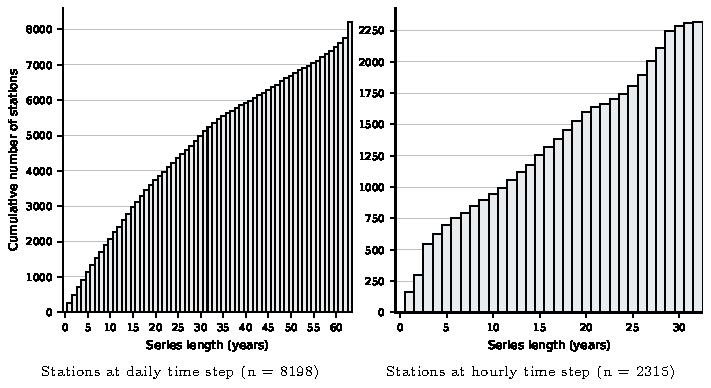
\includegraphics[width=\linewidth]{fig1.pdf}
  \DIFaddendFL \caption{Map showing the computational domain of the AROME model. Shading shows topography at 2.5 km resolution and thin lines indicate the 400 m elevation contour. The letters show the geographical zones cited in the article.}\label{fig:map_domain}
\end{center}
\end{figure}

%DIF < \cite{Caillaud2021} have evaluated the previous version of AROME model forced by ERA-Interim. They show a generally good representation of heavy precipitation events, but several systematic biases are documented. The model tends to underestimate the most intense daily and hourly extremes, particularly for the highest values (>200 mm/d and >40 mm/h). AROME also exhibits seasonal temperature biases: a cold bias in winter--spring, and a warm bias in summer associated with an excess of incoming short-wave radiation linked to underestimated cloud cover. In mountainous areas, the model is too cold and too wet, and snow cover tends to persist unrealistically above roughly 2000 m. Some precipitation-system properties (extent, duration, volume) also remain biased when compared with reference products. 
\DIFdelbegin %DIFDELCMD < 

%DIFDELCMD < \begin{figure}
%DIFDELCMD < \begin{center}
%DIFDELCMD <   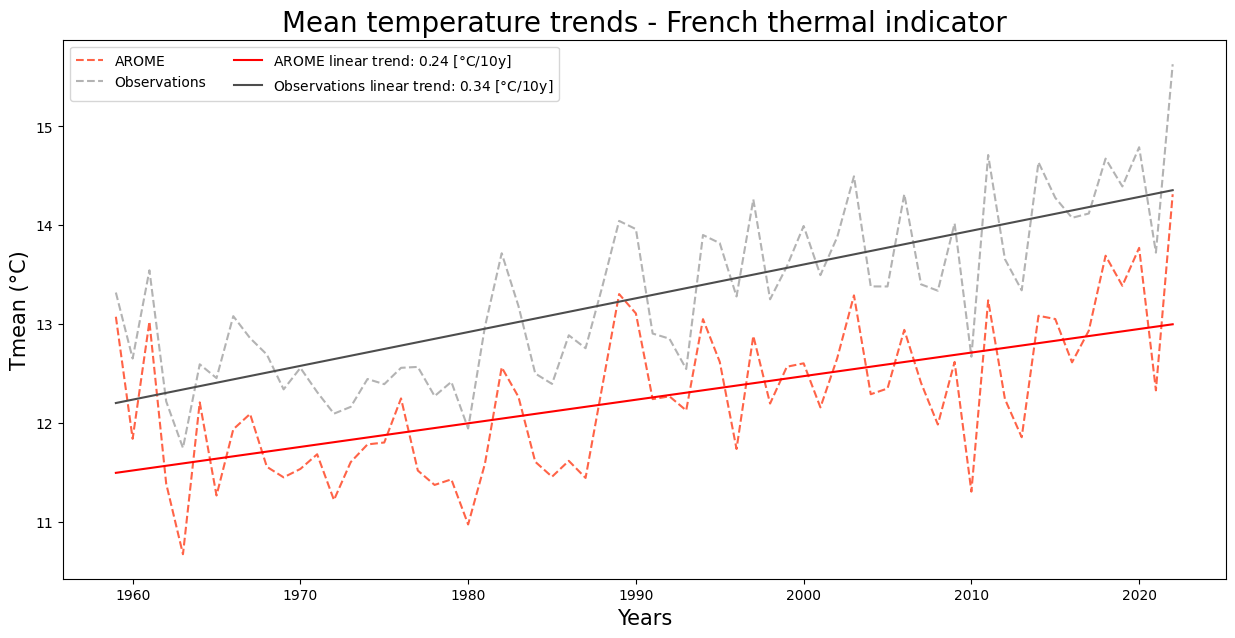
\includegraphics[width=\linewidth]{Trend_TM_ARO_OBS_yea_1959-2022.png}
%DIFDELCMD <   %%%
%DIFDELCMD < \caption{%
{%DIFAUXCMD
\DIFdelFL{Temporal evolution of the annual mean temperature between 1959 and 2022. For the observations, the time-series are computed from the French thermal indicator, i.e. the mean of a given set of 30 stations with homogenised data, which are the reference temperature stations in France \mbox{%DIFAUXCMD
\citep{gibelin-etal-2014}}\hskip0pt%DIFAUXCMD
. For the model, the time-series are computed over the mean of the 30 grid-points that are the closest to the stations. For each time-series, the trend is computed using a linear regression.}}%DIFAUXCMD
%DIFDELCMD < \label{fig:trend_tempe}
%DIFDELCMD < \end{center}
%DIFDELCMD < \end{figure}
%DIFDELCMD < 

%DIFDELCMD < %%%
\DIFdel{It should be noted that temperature trends (cf. Figure~\ref{fig:trend_tempe}) with the AROME model forced by ERA5 are about one-third weaker than observed trends. This implies a dampening of the Clausius-Clapeyron-related component of extreme precipitation trends, which is expected to influence the magnitude of the trends we can detect.
}%DIFDELCMD < 

%DIFDELCMD < %%%
\DIFdelend \section{Methodology}\label{methodology}

The primary objective of this study is to
validate the AROME model (grid points) against stations
over metropolitan France. This is first conducted under
stationary conditions to focus on the climatology (Section \ref{climatology}), then in a non-stationary context to assess the variability and trends in extremes (Section \ref{trends-in-extremes}).

Evaluation is made per year\DIFdelbegin \DIFdel{and season}\DIFdelend \DIFaddbegin \DIFadd{, season, and month}\DIFaddend . Seasons are defined as follows: \textbf{OND}:
October (OCT), November (NOV), December (DEC), \textbf{JFM}: January
(JAN), February (FEB), March (MAR), \textbf{AMJ}: April (APR), May
(MAY), June (JUN), \textbf{JAS}: July (JUL), August (AUG), September
(SEP). The hydrological year (\textbf{YEAR}) is defined as the period
from 1 September of year N to 31 August of year N+1. \DIFaddbegin \DIFadd{The hydrological year (September to August) is used instead of the calendar year, which is standard in French climatology and hydrology. This choice is motivated by the fact that the most intense extreme precipitation events in France, particularly Mediterranean episodes (e.g., Cévenol events), occur during autumn (September–November). Using a calendar year would risk splitting these autumn events across two years, violating the block-independence assumption required for annual maxima GEV modeling.
}\DIFaddend 

\subsection{Climatology of extremes}\label{climatology}

%DIF < \subsubsection{GEV distribution for extremes}\label{gev-distribution-for-extremes}
\DIFdelbegin %DIFDELCMD < 

%DIFDELCMD < %%%
\DIFdelend While descriptive statistics such as mean precipitation or wet day frequency provide useful summaries for overall precipitation, they cannot assess quality of rare occurrence, e.g. of 10 year return events that are exceeded on average only once every 10 years. %Furthermore, the descriptive statistics of Section 3.1 are stationary, thus they cannot inform about potential trends. 
To address
this limitation, we apply extreme value theory (EVT) \citep{coles2001introduction}. This states that, under general conditions, the cumulative distribution function (CDF) of block maxima - e.g. annual maxima - can be approximated by the Generalized Extreme Value (GEV)
distribution.

The GEV distribution is a continuous
probability distribution parameterized by the triplet
\(\theta = (\mu, \sigma, \xi)\) --- respectively the location, scale
(strictly positive), and shape---with the following cumulative
distribution function: \[
F(x;\mu ,\sigma ,\xi) = \exp\left\{-\left[1 + \xi\frac{x - \mu}{\sigma}\right]^{-1/\xi}\right\}, \quad 1 + \xi\frac{x - \mu}{\sigma} > 0
\]

It unifies the three classical distributions Gumbel (\(\xi \to 0\)), Fréchet (\(\xi > 0\)) and Weibull (\(\xi < 0\)) where the shape parameter \(\xi\) determines the tail behavior.

The return level (or quantile of order \(1 - \tfrac{1}{T}\)) of the GEV
distribution corresponds to the threshold value exceeded, on
average, once every \(T\) years. 
Denoting by $F^{-1}$ the quantile function of the GEV, it is given by:

\begin{equation}\label{eq:RLstat}
\mathrm{RL}_{T}
= F^{-1}\!\left(1 - \frac{1}{T}\right)
= \mu + \frac{\sigma}{\xi}
\left[
\left(
-\log\!\left(1 - \frac{1}{T}\right)
\right)^{-\xi}
- 1
\right].
\end{equation}


The GEV parameters $(\mu,\sigma,\xi)$ are estimated by maximum likelihood method for each
spatial location separately, considering the block maxima at a given
location to be independent. This gives a set of parameters $\mu,\sigma,\xi$ and thus
return level estimates from Eq.~\ref{eq:RLstat}.

\subsection{Trends in extremes}\label{trends-in-extremes}

\subsubsection{Non-stationary GEV models}\label{non-stationary-gev}

To consider trends in extremes, the GEV distribution can be made non-stationary
by allowing at least one GEV parameter to vary with time: $\mu(t)$, $\sigma(t)$
and/or $\xi(t)$. Owing to the difficulty of estimating the tail parameter $\xi$,
it is assumed stationary, i.e. $\xi(t) = \xi_0$. Three non-stationary models are
considered:

\[
\begin{array}{c@{\qquad}c@{\qquad}c}
% -------- Column 1 --------
\begin{array}{c}
\begin{aligned}
M_1(\theta_1)\\[-0.2ex]
\theta_1 = (\mu_0, \mu_1, \sigma_0, \xi_0)
\end{aligned}\\[0.4ex]
\begin{cases}
\mu(t) = \mu_0 + \mu_1\, t \\
\sigma(t) = \sigma_0 \\
\xi_0
\end{cases}
\end{array}
&
% -------- Column 2 --------
\begin{array}{c}
\begin{aligned}
M_2(\theta_2)\\[-0.2ex]
\theta_2 = (\mu_0, \sigma_0, \sigma_1, \xi_0)
\end{aligned}\\[0.4ex]
\begin{cases}
\mu(t) = \mu_0 \\
\sigma(t) = \sigma_0 + \sigma_1\, t \\
\xi_0
\end{cases}
\end{array}
&
% -------- Column 3 --------
\begin{array}{c}
\begin{aligned}
M_3(\theta_3)\\[-0.2ex]
\theta_3 = (\mu_0, \mu_1, \sigma_0, \sigma_1, \xi_0)
\end{aligned}\\[0.4ex]
\begin{cases}
\mu(t) = \mu_0 + \mu_1\, t \\
\sigma(t) = \sigma_0 + \sigma_1\, t \\
\xi_0
\end{cases}
\end{array}
\end{array}
\]


Furthermore, based on previous studies that showed trends in extremes in France emerging in the mid-80s
\citep{Blanchet2018,Ribes2019,blanchet-creutin-2022}, we consider the case of a
trend starting at year $t_{+}=1985$, leading to the three models
$M_{1}^{*}$, $M_{2}^{*}$, and $M_{3}^{*}$. For example, in $M_{1}^{*}$:

\[
\mu(t)=
\begin{cases}
\mu_{0} & \text{if } t \le 1985,\\[4pt]
\mu_{0} + \mu_{1}(t-1985) & \text{if } t \ge 1985.
\end{cases}
\]

Figure \ref{fig:illustrGEV} illustrates the case of a non stationary GEV with trends in $\mu$ and $\sigma$ starting in 1985 (corresponding to $M_3^*$), with the corresponding GEV densities and associated return level plots for several years.

\begin{figure}
    \centering
    \DIFdelbeginFL %DIFDELCMD < 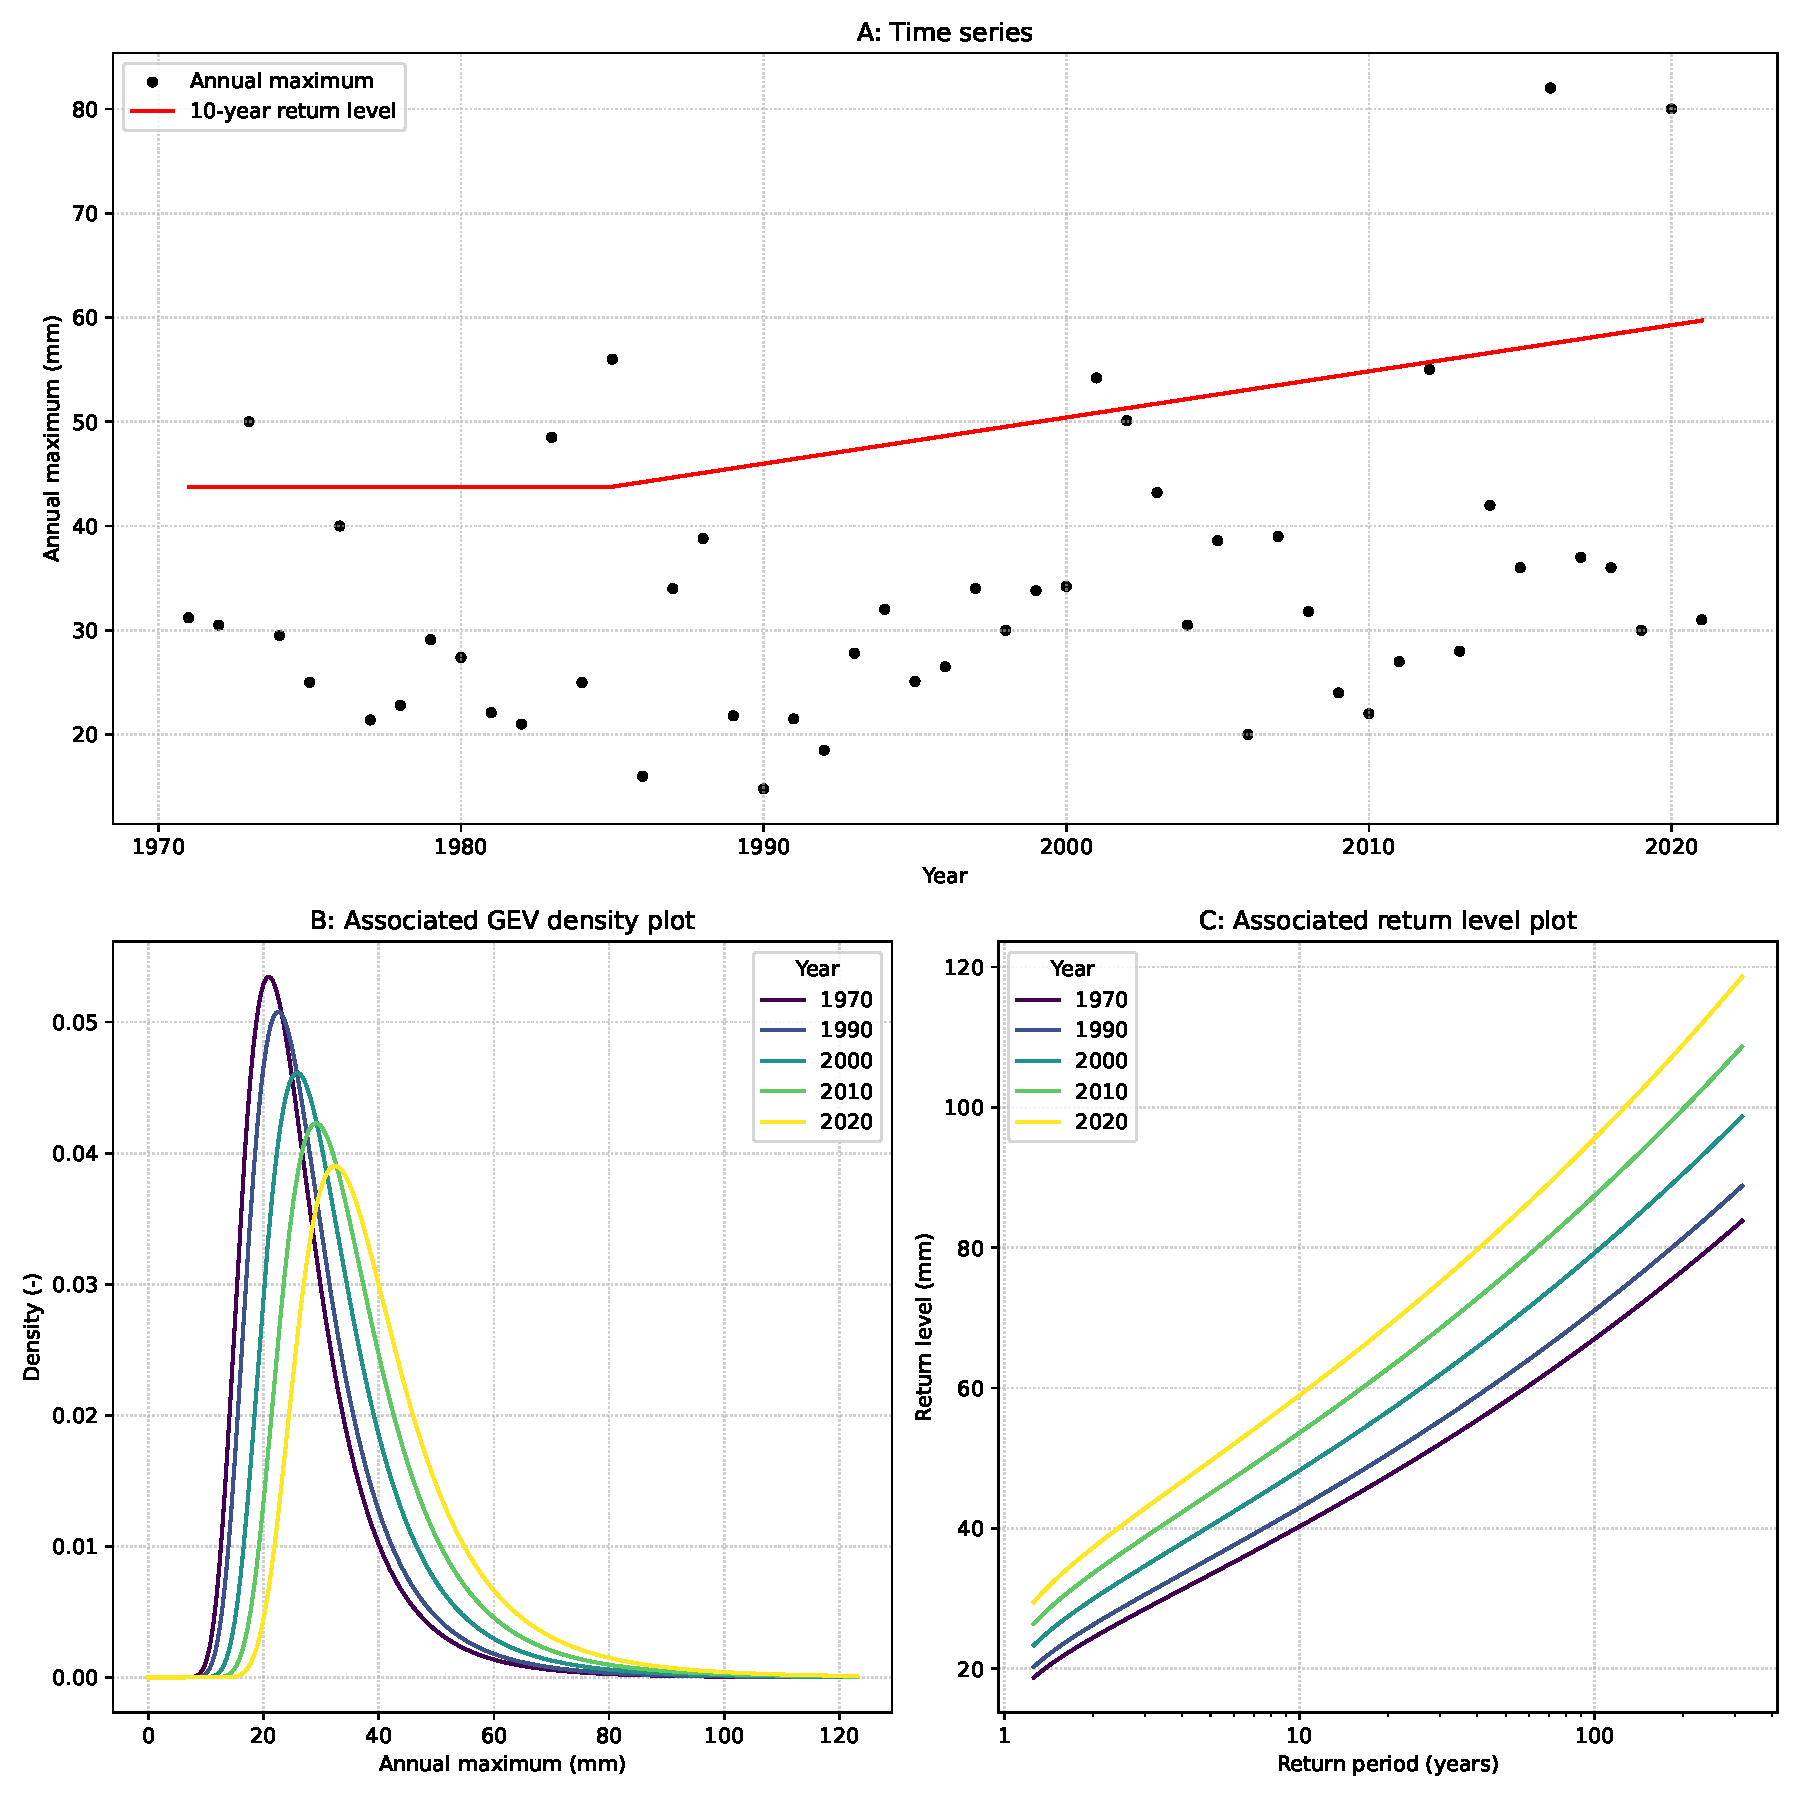
\includegraphics[width=\textwidth]{annexe3.pdf}
%DIFDELCMD <     %%%
\DIFdelendFL \DIFaddbeginFL 
\includegraphics[width=\textwidth]{fig2.pdf}
    \DIFaddendFL \caption{Influence of a trend in the $\mu$ and $\sigma$ parameters for a time series of annual maxima (Example: Station 45330001 located at 48.09$^\circ$ N, 1.94$^\circ$ E). \DIFaddbeginFL \DIFaddFL{This figure illustrates an example of the $M_{3}^{*}$ model showing a positive trend. }\DIFaddendFL (a) Time series (black dots) with the 10-year return level (red line); (b) GEV densities for selected years between 1970 (purple) and 2020 (yellow); (c) Associated return level curves.} \label{fig:illustrGEV}
\end{figure}

This gives in total six non-stationary models, in addition to the stationary model denoted ($M_0$), which corresponds to $\mu(t)=\mu_0$, $\sigma(t)=\sigma_0$, and $\xi(t)=\xi_0$. Although the starting year $t_{+}=1985$ will be hold fixed below, considering starting year a few years before or after does not change the main results of this study (not shown).

\subsubsection{Model selection}\label{model-selection}

For each model, the GEV parameters $\theta$ are estimated by maximum likelihood method for each
spatial location separately. 
At each spatial point, we thus have seven estimated models
\(M_0, M_1, M_2, M_3, M_1^\ast, M_2^\ast\), and \(M_3^\ast\) that we temporarily rename $M_{0}$ to $M_{6}$. \DIFaddbegin \DIFadd{For the hourly series (1990--2022), because all observations start after 1985, the breakpoint models $M^\ast$ are equivalent to the standard linear models $M$, and the selection procedure defaults to the latter. }\DIFaddend We apply for each non-stationary model $M_{j}$, $j \ge 1$, a likelihood ratio test to compare the goodness of fit of $M_{j}$ to that of the stationary model $M_{0}$, accounting for their respective number of parameters to avoid overfitting. The test is based on computing the statistics $\Lambda_{j}=2\bigl(\ell_{j}-\ell_{0}\bigr)$, where $\ell$ are the maximum likelihood values. Under the null hypothesis that the maxima are stationary, the statistics $\Lambda_{j}$ follows a $\chi^2$ with $k$ degress of freedom, with $k$ equal the difference in the number of parameters between $M_j$ and $M_0$. 

 Let $p_{j}$ be the corresponding $p$-value.  If $p_{j} \le 10\%$, the model $M_{j}$ is considered to perform better than $M_{0}$, otherwise $M_{0}$ is selected. If several models $M_{j}$ are preferred to $M_{0}$, we apply the following procedure: 1) if either $M_{3}$ or $M_{3}^{*}$ are preferred to $M_{0}$, we select among these two models that with the smallest $p$-value among $p_{3}$ and $p_{3}^{*}$; 2) otherwise, we select among $M_{1}$, $M_{1}^{*}$, $M_{2}$, $M_{2}^{*}$ that with the smallest $p$-value among $p_{1}$, $p_{1}^{*}$, $p_{2}$, $p_{2}^{*}$.

This two-step process prioritizes models with simultaneous temporal
effects on \(\mu\) and \(\sigma\) when statistically justified, ensuring
complexity is introduced only when it provides plus-value. In the rest of the article, only the selected model is considered at each location (grid point or station). However, for the evaluation of 10-year return levels as a climatological metric, we consistently rely on the stationary model ($M_0$). 

\subsubsection{Trend in return level}\label{return-level}

For a non-stationary GEV with parameters $\mu(t)$, $\sigma(t)$ and $\xi_{0}$, the $T$-year return level is still given by Eq. \ref{eq:RLstat} but it is now a function $RL_T(t)$ of the year $t$. \DIFaddbegin \DIFadd{In this study, we focus on the 10-year return level ($\mathrm{RL}_{10}$) as the primary metric for extreme precipitation. Our daily series (63 years) and hourly series (33 years) provide sufficient data for its robust estimation. As a sensitivity check, trends in $\mathrm{RL}_{2}$ and $\mathrm{RL}_{5}$ show the same regional patterns as $\mathrm{RL}_{10}$ (daily: $r=0.86$--$0.99$ among significant stations; hourly: $r=0.79$--$0.98$), confirming that the detected signals are robust and not driven by GEV fitting uncertainty.
}\DIFaddend 

Owing to the linear form of $\mu(t)$ and $\sigma(t)$ in the considered
non-stationary models, return levels are linear functions of time in
models $M_{1}$, $M_{2}$, and $M_{3}$, and linear only after 1985 in the
breakpoint models $M_{1}^{*}$, $M_{2}^{*}$, and $M_{3}^{*}$. In the
stationary model $M_{0}$, return levels are of course constant over time.
For the non-stationary models, the relative trend in the $T$-year return
level (\%) over the most recent 30-year period (between 1992 and 2022) is computed as

\[
\mathrm{RelTrend} =
\frac{\mathrm{RL}_{T}(2022)-\mathrm{RL}_{T}(1992)}{\mathrm{RL}_{T}(1992)}.
\]

It is obviously $0$ if the stationary model has been selected.

\subsubsection{Confidence intervals for the return levels}\label{maximu-likelihood-estimation-and-confidence-intervales}

Noting that the
$T$-year return level function can be written as
$\mathrm{RL}_{T}(t)=\mathrm{RL}_{T,0}+\mathrm{RL}_{T,1}\, t$
for models $M_{1}$, $M_{2}$, $M_{3}$ and as
\[
\mathrm{RL}_{T}(t)=
\begin{cases}
\mathrm{RL}_{T,0} & \text{if } t \leq 1985,\\[4pt]
\mathrm{RL}_{T,0}+\mathrm{RL}_{T,1}(t-1985) & \text{if } t>1985,
\end{cases}
\]
for models $M_{1}^{*}$, $M_{2}^{*}$, $M_{3}^{*}$,
confidence intervals for the trend coefficient $\mathrm{RL}_{T,1}$ are obtained
by profiling the likelihood with respect to $\mathrm{RL}_{T,1}$ \citep{coles2001introduction}. If
the $90\%$ confidence interval of $\mathrm{RL}_{T,1}$ does not contain $0$, the
$T$-year return level trend is significant at level $10\%$.



%DIF < \subsection{Assessing the agreement between AROME and the stations}\label{assessing}
%DIF < 
%DIF < We evaluate the agreement between each
%DIF < Météo-France station is matched to the corresponding AROME grid point
%DIF < (2.5 km × 2.5 km) based on its spatial location. This
%DIF < correspondence allows calculating the Pearson correlation (\(r\)) and
%DIF < mean error (\(ME\)) between observed and simulated statistics.
\DIFaddbegin \subsection{\DIFadd{Assessing the agreement between AROME and the stations}}\label{assessing}
\DIFaddend 

\DIFaddbegin \DIFadd{To evaluate the CNRM-AROME model against observations, each Météo-France station is matched to the closest model grid point (2.5 km $\times$ 2.5 km) based on its geographic location. This pairing allows assessing the spatial and temporal coherence of simulated fields against raingauge measurements.
}

\DIFadd{We assess the model's agreement using three main metrics:
}\begin{enumerate}
    \item \textbf{\DIFadd{Pearson correlation coefficient ($r$):}} \DIFadd{Used to quantify the spatial consistency between observed and simulated fields across all station locations.
    }\item \textbf{\DIFadd{Mean Error ($ME$, or absolute bias):}} \DIFadd{Measures the average difference between the simulated and observed statistics, defined as:
    }\begin{equation}
        \DIFadd{ME = \frac{1}{n}\sum_{i=1}^{n} (Y_{i,\text{AROME}} - Y_{i,\text{OBS}})
    }\end{equation}
    \DIFadd{where $Y_i$ represents the climatological or trend statistic computed at station $i$ (or its closest model grid point) and $n$ is the total number of compared stations.
    }\item \textbf{\DIFadd{Relative Bias ($RB$, \%):}} \DIFadd{Expresses the bias as a percentage of the observed baseline, which is particularly useful for comparing regions with highly contrasted precipitation baselines:
    }\begin{equation}
        \DIFadd{RB = 100 \times \frac{\sum_{i=1}^{n} (Y_{i,\text{AROME}} - Y_{i,\text{OBS}})}{\sum_{i=1}^{n} Y_{i,\text{OBS}}} = 100 \times \frac{ME}{\bar{Y}_{\text{OBS}}}
    }\end{equation}
    \DIFadd{where $\bar{Y}_{\text{OBS}}$ is the mean of the observed values across all compared stations.
}\end{enumerate}

\DIFadd{These metrics are calculated for five core precipitation indices: the annual frequency of wet days (daily precipitation exceeding 1\,mm), the mean annual total precipitation, the daily and hourly 10-year return levels, and the relative trends in daily and hourly 10-year return levels. Climatological indices are evaluated in a stationary framework, whereas relative trends are obtained from the estimated non-stationary GEV distributions (cf. Sect.~\ref{non-stationary-gev}). In the latter case, we do not compute the relative bias as relative trends are already \%.
}

\DIFaddend \section{Results}\label{results}

We begin by evaluating, grid point by grid point, the ability of AROME
to reproduce the precipitation regime observed by Météo-France stations.
This initial stationary evaluation allows assessing the quality of the extreme-value climatology before examining return-level trends.

\subsection{Evaluation of the precipitation climatology of AROME}
\label{evaluation-of-the-precipitation-climatology-by-arome}

Figure~\ref{fig:map_clim} provides a spatial comparison of the precipitation climatology between AROME and Météo-France stations. In addition to the 10-year return level assessing quality of extremes, we show two descriptive statistics assessing the overall climatology of precipitation: the mean number of wet days per year (precipitation exceeding 1 mm) and the mean annual total precipitation. Across all indicators, AROME reproduces the large-scale spatial structures with high spatial correlations: matching the station locations to their closest grid points, Pearson correlation \emph{r} = 0.95 for the annual frequency of precipitation days, \emph{r} = 0.94 for annual cumulative precipitation, \emph{r} = 0.95 for the daily 10-year return level, and a lower correlation of \emph{r} = 0.78 for the hourly 10-year return level. The model correctly captures the main climatic gradients of France: dryness of the Rhône valley and the Mediterranean coast (50-70 wet days per year, annual totals no more than 550 mm per year) contrasting with the wetness of the mountain ranges (Alps, Pyrenees, Massif Central, Vosges, Jura; 140--160 wet days per year, annual totals up to more than 1800 mm per year). The model also reproduces the localization of the largest extremes along the Massif Central ridge and to a lesser extent in the Rhône valley and along the Mediterranean coast at both daily and hourly scales.

\begin{figure}[htbp]
    \centering
    
\includegraphics[width=\textwidth]{fig3.pdf}
    %DIF < \setcounter{figure}{2}
    \caption{Climatology of the AROME \DIFdelbeginFL \DIFdelFL{model }\DIFdelendFL \DIFaddbeginFL \DIFaddFL{simulations }\DIFaddendFL (first row), Météo-France stations (second row), \DIFdelbeginFL \DIFdelFL{and }\DIFdelendFL the AROME--Station \DIFaddbeginFL \DIFaddFL{absolute }\DIFaddendFL difference (third row), \DIFaddbeginFL \DIFaddFL{and the relative bias (fourth row), }\DIFaddendFL with the spatial correlation between the stations and their closest grid points ($r$), the bias ($ME$ \DIFaddbeginFL \DIFaddFL{or relative bias $RB$ in bold}\DIFaddendFL ) and the number of stations compared (\DIFdelbeginFL \DIFdelFL{n}\DIFdelendFL \DIFaddbeginFL \DIFaddFL{$n$}\DIFaddendFL ). The statistics of the three first columns are derived from daily data from 1959 to 2022. The last \DIFdelbeginFL \DIFdelFL{columns }\DIFdelendFL \DIFaddbeginFL \DIFaddFL{column }\DIFaddendFL uses hourly data from 1990 to 2022. The contour lines show the 400 and 800\DIFaddbeginFL \DIFaddFL{\,}\DIFaddendFL m \DIFaddbeginFL \DIFaddFL{elevation }\DIFaddendFL isolines. \DIFdelbeginFL \DIFdelFL{To ease visualization, colour }\DIFdelendFL \DIFaddbeginFL \DIFaddFL{Colour }\DIFaddendFL scales are symmetrically saturated\DIFdelbeginFL \DIFdelFL{above the 99.9th percentile for the number of days and the 99th percentile for annual and 10-year return level precipitation)}\DIFdelendFL . \DIFaddbeginFL \DIFaddFL{Station markers have uniform size; zero bias is shown as a clearly visible grey fill.}\DIFaddendFL }\label{fig:map_clim}
\end{figure}

Despite this overall agreement, the difference maps reveal structured regional biases. For precipitation frequency, AROME shows little mean bias (+6 days/year) but local excesses above +30 days/year in the Massif Central and Pyrenees, while negative biases (-10 to -30 days/year) appear in the Northern Alps, Brittany, and the Vosges. For annual cumulative precipitation, the mean bias is very small (+11 mm/year) but regional discrepancies reach more than +300 mm per year along the Pyrenean ridge and Northern Alps, and -100 to -400 mm per year from the Northern Pré-Alps to the Vosges. For daily 10-year return level, AROME shows almost no mean bias (-2 mm) but it spreads the extremes too widely around the Massif Central ridge, giving local deficits of -10 to -20 mm along the ridge where the station extremes are the largest and +10 to +30 mm over the Massif Central Plateau. Overestimation is also visible in the Northern Alps and the Pyrenees.  At the hourly scale, AROME strongly underestimates the 10-year return levels (\(-6.37\) mm, \(-23.30\)\,\%), with widespread deficits of \(-5\) to \(-20\) mm over most of France, especially in the southern Massif Central and the Rhône Valley.

The good performance of AROME for the frequency of wet days, the annual precipitation and the daily extremes is found across all seasons (see Figure~\ref{fig:correlation_clim} for an overall view and Figures \ref{ann:map_trend_daily} and \ref{ann:map_trend_hourly} for seasonal maps of extremes), despite a slight loss in performance in spring and summer for the extremes (AMJ to JAS, correlation around $0.9$). Performance is lower for hourly extremes across all seasons and particularly in spring where correlation drops to 0.38.

\begin{figure}[htp]
\centering
    
\includegraphics[width=0.85\textwidth]{fig4.pdf}
    %DIF < \captionsetup{type=figure}
    %DIF < \setcounter{figure}{3}% prochaine légende = Figure 4
    \caption{\DIFdelbeginFL \DIFdelFL{Spatial correlations }\DIFdelendFL \DIFaddbeginFL \DIFaddFL{Seasonal synthesis }\DIFaddendFL of \DIFaddbeginFL \DIFaddFL{the }\DIFaddendFL climatological \DIFdelbeginFL \DIFdelFL{indices }\DIFdelendFL \DIFaddbeginFL \DIFaddFL{agreement }\DIFaddendFL between the AROME \DIFdelbeginFL \DIFdelFL{model }\DIFdelendFL \DIFaddbeginFL \DIFaddFL{simulations }\DIFaddendFL and Météo-France stations \DIFdelbeginFL \DIFdelFL{at daily }\DIFdelendFL \DIFaddbeginFL \DIFaddFL{for the four precipitation indices: (a) spatial Pearson correlation ($r$) }\DIFaddendFL and \DIFdelbeginFL \DIFdelFL{hourly scales }\DIFdelendFL \DIFaddbeginFL \DIFaddFL{(b) relative bias ($RB$, in \%) }\DIFaddendFL depending on the season.}\label{fig:correlation_clim}
\end{figure}

In summary, AROME shows a good representation of the climatology of precipitation extremes that encourages us to continue evaluation on trends, keeping however in mind that hourly extremes are \DIFdelbegin \DIFdel{poorly represented }\DIFdelend \DIFaddbegin \DIFadd{systematically underestimated by the model throughout the year (especially during spring and summer) and exhibit a lower spatial agreement }\DIFaddend in spring.

\subsection{Evaluation of extreme precipitation
trends}\label{evaluation-of-extreme-precipitation-trends}

\subsubsection{Daily}

At the \DIFdelbegin \DIFdel{daily }\DIFdelend \DIFaddbegin \DIFadd{hydrological year scale, the stationary model is selected for about two-thirds of the stations. For the remaining one-third, significant changes in the GEV distributions are observed, with nearly equal proportions of linear trend model ($M$) and breakpoint models ($M^{*}$). AROME
model exhibit similar proportions. At the seasonal scale, the only notable difference occurs in winter, where the linear model is slightly more frequent than the breakpoint model (22\% vs. 13\%). Before analyzing trends in daily return levels, we verified the consistency of GEV-estimated trends in the mean against those obtained via a simple linear regression on observed annual maxima. This preliminary check shows a very strong spatial and quantitative agreement (Pearson correlation $r = 0.86$ for absolute trends, $r = 0.88$ for relative trends), confirming the robustness of the statistical fits.
}

\DIFadd{At the daily }\DIFaddend scale, station-based trends in the 10-year return level (Figure~\ref{fig:map_daily_trend}) show spatially coherent but region-dependent signals across France over 1959--2022. For the hydrological year (YEAR), we see a clear reinforcement along the Rhône Valley (+5\% to \(>+30\%\)) and in the southern Alps (+20\% to +30\%). Elsewhere, trends are weak, of mixed sign, and often not significant, supporting a seasonal breakdown. Autumn (OND) shows a similar pattern in trends as the annual scale, with the exception of the Paris area that shows a decrease (-5 to -20\%). In winter (JFM), France is cut in three with a diagonal of decrease from the Mediterranean coast to the Atlantic coast (-10 to -40\%) and mainly increases elsewhere. Spring (AMJ) is characterized by a more spatially uniform positive trend over much of the country, with local increases exceeding +35\%. Summer (JAS), shows predominantly negative trends in the southern half of France, apart in the Rhône valley, with an accentuated decrease along the Mediterranean coast (up to -40\%) and mainly positive trends in the northern half.

AROME reproduces the broad spatial organization of these daily-scale patterns but generally underestimates their amplitudes (negative bias). For the hydrological year, the model partly captures the significant increase in the Southern Alps, albeit with weaker intensities, and does not reproduces the Rhône Valley reinforcement observed in the stations. Autumn is the season when trend patterns are best represented ($r=0.40$). AROME correctly identifies the positive signal in the Rhône valley and the negative trends in the Paris area, although it barely sees the decrease in the northern Alps. In winter, the model barely retrieves the diagonal of decrease from the Mediterranean to the Atlantic coast and it misses the decrease over the Alps. All the largest trends are anyway less marked. In spring, AROME produces weak and poorly organized signals and fails to reproduce the widespread positive trends measured by the stations. In summer, the model correctly identifies a general negative tendency over the souther half of France but does not see the increase over the Rhône valley and the northern half of France. Overall, AROME \DIFaddbegin \DIFadd{moderately }\DIFaddend captures the large-scale signs and structure of daily return-level trends but tends to underestimate both their intensity and spatial coherence.

\begin{figure}[htbp]
    
\includegraphics[width=0.85\textwidth]{fig5.pdf}
    \caption{Relative trends over \DIFdelbeginFL \DIFdelFL{the last thirty years ending in 2022 }\DIFdelendFL \DIFaddbeginFL \DIFaddFL{1959--2022 }\DIFaddendFL (\%) in the 10-year return level of daily precipitation for AROME (left) and Météo-France stations (right). \DIFdelbeginFL \DIFdelFL{The correlation }\DIFdelendFL \DIFaddbeginFL \DIFaddFL{Display conventions: non-significant stations as open circles }\DIFaddendFL (\DIFdelbeginFL \DIFdelFL{$r$}\DIFdelendFL \DIFaddbeginFL \DIFaddFL{white fill}\DIFaddendFL )\DIFdelbeginFL \DIFdelFL{, the number of stations compared }\DIFdelendFL \DIFaddbeginFL \DIFaddFL{; significant trends close to zero as filled grey }\DIFaddendFL (\DIFdelbeginFL \DIFdelFL{n}\DIFdelendFL \DIFaddbeginFL \DIFaddFL{dark outline}\DIFaddendFL )\DIFdelbeginFL \DIFdelFL{, and }\DIFdelendFL \DIFaddbeginFL \DIFaddFL{; significant non-zero trends coloured on }\DIFaddendFL the \DIFdelbeginFL \DIFdelFL{bias }\DIFdelendFL \DIFaddbeginFL \DIFaddFL{map scale }\DIFaddendFL (\DIFaddbeginFL \DIFaddFL{uniform marker size); non-significant AROME grid cells not displayed. Metrics ($r$, $n$, }\DIFaddendFL $ME$) are computed on \DIFdelbeginFL \DIFdelFL{the stations with }\DIFdelendFL significant trends \DIFaddbeginFL \DIFaddFL{only}\DIFaddendFL .\DIFdelbeginFL \DIFdelFL{These results are derived by fitting, at each location, the selected GEV model to daily precipitation maxima from 1959 to 2022. The contour lines show the 400 and 800 m isolines. To ease visualization, colour scales are symmetrically saturated using a 99\% threshold. All maps are clipped to this common percentile range. Only statistically significant trends are shown, non-significant trends are set to zero.}\DIFdelendFL }\label{fig:map_daily_trend}
%DIF <   \centering
%DIF <   \nolinenumbers
%DIF <   %\setcounter{figure}{5}
%DIF <   \begin{overpic}[width=\linewidth]{fig5.pdf}
%DIF <     % Ajuster 73,6 (x,y en %) et la largeur 0.25\linewidth
%DIF <     \put(53,8){%
%DIF <       \colorbox{white}{%
%DIF <         \parbox{0.42\linewidth}{\justifying\footnotesize
%DIF <           {\figurename~\thefigure} --- Relative trends over the last thirty years ending in 2022 (\%) in the 10-year return level of daily precipitation for AROME (left) and Météo-France stations (right), with the correlation ($r$), the number of stations compared (n), and the bias ($ME$). These results are derived by fitting, at each location, the selected GEV model to daily precipitation maxima from 1959 to 2022. The contour lines show the 400 and 800 m isolines. To ease visualization, colour scales are symmetrically saturated using a 99\% threshold. All maps are clipped to this common percentile range. Only statistically significant trends are shown, non-significant trends are set to zero.%
%DIF <         }%
%DIF <       }%
%DIF <     }
%DIF <   \end{overpic}
  %DIF <  évite une seconde légende visible mais garde la cohérence des flottants
%DIF <   \captionsetup{labelformat=empty}
%DIF <   \caption{}\label{fig:map_daily_trend}
\end{figure}
%DIF < \linenumbers

\subsubsection{Hourly}

\DIFaddbegin \DIFadd{Similarly to the daily scale, we verified the consistency of GEV hourly trends by comparing GEV-estimated trends in the mean to linear regression trends of observed annual maxima. Despite the shorter record length and the higher noise level of sub-daily extremes, we find a robust agreement (Pearson correlation $r = 0.72$ for absolute trends, $r = 0.70$ for relative trends).
}

\DIFaddend At the hourly scale (Figure~\ref{fig:map_hourly_trend}), station-based trends in the 10-year return level over 1990--2022 are markedly more heterogeneous, noisy, and locally more extreme than their daily counterparts (Figure~\ref{fig:map_daily_trend}), with significant trends ranging $[-50\%, +100\%]$ versus $[-30\%, +30\%]$ at the daily scale. Most of the significant trends are highly positive.  Though noisier than at daily scale, these trends are robust in the sense that they are not produced by a single year. Removing the overall maxima of each station and fitting the GEV distributions on these new series gives slightly lower trends for the positive trends and slightly larger trends for the negative ones (Figure \ref{ann:comparaison_trend}) - which was expected since the largest value is omitted - but the magitudes and patterns remain close. Over the hydrological year, \DIFdelbegin \DIFdel{almost no trend }\DIFdelend \DIFaddbegin \DIFadd{no clear spatial pattern of trends }\DIFaddend is found apart in few isolated stations where trends reach $\pm 50\%$ and occasionally exceed $+100\%$. \DIFaddbegin \DIFadd{At the hydrological year scale, the stationary model $M_0$ is selected for 74.2\% of the stations, and standard linear trend models ($M$) for 25.8\% (compared to 75.1\% and 24.9\% for the AROME simulations, respectively). }\DIFaddend Seasonally, the signals remain highly contrasted. In autumn, a pronounced positive pattern emerges along the Mediterranean coast, locally approaching $+100\%$. In winter, no \DIFdelbegin \DIFdel{trend }\DIFdelend \DIFaddbegin \DIFadd{clear spatial pattern of trends }\DIFaddend is found apart at some isolated stations spread over western France, the eastern Pyrenees and the Rhône valley, where strong increases of up to $+100\%$ are found. Spring is the only season when a quite coherent pattern is found. Stations exhibit widespread and very strong increases across much of the country, frequently above $+60\%$ and locally approaching $+100\%$. In summer, spatial variability reaches its maximum, with trends spanning the full range from $-100\%$ to $+100\%$, particularly in the Rhône Valley. These patterns reflect both the strong local variability of convective extremes and the limited length of the hourly record, which jointly hinder the emergence of a clear regional-scale climate signal.

\begin{figure}[htbp]
    
\includegraphics[width=0.85\textwidth]{fig6.pdf}
    \caption{Relative trends over \DIFdelbeginFL \DIFdelFL{the last thirty years ending in 2022 }\DIFdelendFL \DIFaddbeginFL \DIFaddFL{1990--2022 }\DIFaddendFL (\%) in the 10-year return level of hourly precipitation for AROME (left) and Météo-France stations (right)\DIFdelbeginFL \DIFdelFL{, with the correlation }\DIFdelendFL \DIFaddbeginFL \DIFaddFL{. Display conventions: non-significant stations as open circles }\DIFaddendFL (\DIFdelbeginFL \DIFdelFL{$r$}\DIFdelendFL \DIFaddbeginFL \DIFaddFL{white fill}\DIFaddendFL )\DIFdelbeginFL \DIFdelFL{, the number of stations compared }\DIFdelendFL \DIFaddbeginFL \DIFaddFL{; significant trends close to zero as filled grey }\DIFaddendFL (\DIFdelbeginFL \DIFdelFL{n}\DIFdelendFL \DIFaddbeginFL \DIFaddFL{dark outline}\DIFaddendFL )\DIFdelbeginFL \DIFdelFL{, and }\DIFdelendFL \DIFaddbeginFL \DIFaddFL{; significant non-zero trends coloured on }\DIFaddendFL the \DIFdelbeginFL \DIFdelFL{bias }\DIFdelendFL \DIFaddbeginFL \DIFaddFL{map scale }\DIFaddendFL (\DIFdelbeginFL \DIFdelFL{$ME$}\DIFdelendFL \DIFaddbeginFL \DIFaddFL{uniform marker size}\DIFaddendFL )\DIFaddbeginFL \DIFaddFL{; non-significant AROME grid cells not displayed. Metrics ($r$}\DIFaddendFL , \DIFdelbeginFL \DIFdelFL{filtering }\DIFdelendFL \DIFaddbeginFL \DIFaddFL{$n$, $ME$) are computed }\DIFaddendFL on \DIFdelbeginFL \DIFdelFL{the stations with }\DIFdelendFL significant trends \DIFdelbeginFL \DIFdelFL{. These results are derived by fitting}\DIFdelendFL \DIFaddbeginFL \DIFaddFL{only}\DIFaddendFL , \DIFdelbeginFL \DIFdelFL{at each location, the selected GEV model to hourly precipitation maxima from 1990 to 2022. The contour lines show the 400 and 800 m isolines. To ease visualization, colour scales are symmetrically saturated using a }\DIFdelendFL \DIFaddbeginFL \DIFaddFL{with }\DIFaddendFL 90\% \DIFdelbeginFL \DIFdelFL{threshold}\DIFdelendFL \DIFaddbeginFL \DIFaddFL{colour-scale saturation}\DIFaddendFL .\DIFdelbeginFL \DIFdelFL{All maps are clipped to this common percentile range. Only statistically significant trends are shown, non-significant trends are set to zero.}\DIFdelendFL }\label{fig:map_hourly_trend}
%DIF <   \centering
%DIF <   \nolinenumbers
%DIF <   %\setcounter{figure}{6}
%DIF <   \begin{overpic}[width=\linewidth]{fig6.pdf}
%DIF <     % Ajuster 73,6 (x,y en %) et la largeur 0.25\linewidth
%DIF <     \put(53,8){%
%DIF <       \colorbox{white}{%
%DIF <         \parbox{0.42\linewidth}{\justifying\footnotesize
%DIF <           {\figurename~\thefigure} --- Relative trends over the last thirty years ending in 2022 (\%) in the 10-year return level of hourly precipitation for AROME (left) and Météo-France stations (right), with the correlation ($r$), the number of stations compared (n), and the bias ($ME$). These results are derived by fitting, at each location, the selected GEV model to hourly precipitation maxima from 1990 to 2022. The contour lines show the 400 and 800 m isolines. To ease visualization, colour scales are symmetrically saturated using a 90\% threshold. All maps are clipped to this common percentile range. Only statistically significant trends are shown, non-significant trends are set to zero.%
%DIF <         }%
%DIF <       }%
%DIF <     }
%DIF <   \end{overpic}
%DIF <   % évite une seconde légende visible mais garde la cohérence des flottants
%DIF <   \captionsetup{labelformat=empty}
%DIF <   \caption{}%
\end{figure}


AROME only partially reproduces these hourly-scale patterns. Across all seasons, the model simulates weak and spatially inconsistent signals and fails to capture the most pronounced positive trends seen in the station data. For the hydrological year, spatial correlation between AROME and stations remains low ($r \approx 0.12$), and seasonal correlations are close to zero for several seasons. Mean biases are substantial and of varying sign, with values reaching \DIFdelbegin \DIFdel{$ME = +84.7\%$ }\DIFdelend \DIFaddbegin \DIFadd{$ME = -84.7\%$ }\DIFaddend in spring and $ME = -28.4\%$ in summer. While AROME occasionally recovers the sign of the observed trends in some regions, it generally does not reproduce their fine-scale spatial organization or amplitude.

%DIF < \linenumbers
\DIFaddbegin \subsubsection{\DIFadd{Monthly refinement}}
\DIFaddend 

%DIF < \subsubsection{Monthly refinement}
\DIFdelbegin %DIFDELCMD < 

%DIFDELCMD < %%%
%DIF < \paragraph{Spatial representation (Figure~7).} 
\DIFdelend The monthly analysis (Figure~\DIFdelbegin \DIFdel{\ref{fig:map_monthly_trend}}\DIFdelend \DIFaddbegin \DIFadd{\ref{fig:correlation_trend}}\DIFaddend ) further highlights the specificity of convective regimes and the strong temporal concentration of some signals. \DIFdelbegin \DIFdel{Station data show that hourly 10-year return level trends are not uniformly distributed }\DIFdelend \DIFaddbegin \DIFadd{Figure~\ref{fig:correlation_trend}a compares the monthly median GEV relative trends at Météo-France stations and the corresponding AROME grid points (side-by-side subpanels). At the daily scale, station median trends remain moderate }\DIFaddend throughout the year\DIFdelbegin \DIFdel{but cluster in a few key months. In late winter, strong increases emerge over the Rhône Valley and the Mediterranean coast in February}\DIFdelend \DIFaddbegin \DIFadd{, ranging from $-16.27\%$ in September to $+14.05\%$ in April/May. In contrast, station-based hourly GEV trends show far larger values concentrated in specific convective windows, with monthly medians reaching $+43.28\%$ in February, $+28.26\%$ in March}\DIFaddend , \DIFdelbegin \DIFdel{while Marchextends these trends all along the western Mediterranean arc. In late autumn, November exhibits substantial increases on the eastern Mediterranean coast (Azur region). In early summer, Junedisplays the clearest signal with widespread positive trends over almost all of France, with local values exceeding $+150\%$. }%DIFDELCMD < 

%DIFDELCMD < %%%
\DIFdel{AROME reproduces partly the enhanced activity of some months but it }\DIFdelend \DIFaddbegin \DIFadd{$+101.86\%$ in June, $+53.88\%$ in October, and $+30.09\%$ in December. AROME reproduces the positive sign of these monthly trend peaks but systematically }\DIFaddend underestimates their magnitude. \DIFdelbegin \DIFdel{The model reproduces the existence of positive signals in February, March, November, and }\DIFdelend \DIFaddbegin \DIFadd{For instance, in }\DIFaddend June, \DIFdelbegin \DIFdel{consistent with the station-based identification of convectively active months.
However, the simulated trends are often weaker by a factor of two and display inconsistent spatial localization compared to observations, as reflected by the very low spatial correlations for some }\DIFdelend \DIFaddbegin \DIFadd{AROME simulates a median hourly GEV trend of $+17.70\%$ (against $+101.86\%$ for stations), and in February, it simulates $+11.46\%$ (against $+43.28\%$ for stations).
}

\DIFadd{This systematic underestimation is reflected in the monthly mean errors ($ME$) between the stations and the corresponding AROME grid points shown in Figure~\ref{fig:correlation_trend}b, with large negative values at the hourly scale during convective }\DIFaddend months (e.g.\DIFdelbegin \DIFdel{\ $r = 0.08$ in June)}\DIFdelend \DIFaddbegin \DIFadd{, $ME = -41.6\%$ in February, $ME = -13.6\%$ in March, and $ME = -82.2\%$ in June), whereas daily mean errors remain much smaller (e.g., $ME = 0.2\%$ in January and $ME = 4.3\%$ in March)}\DIFaddend .

\DIFdelbegin %DIFDELCMD < \begin{figure}[htp]
%DIFDELCMD < \centering
%DIFDELCMD <     
\includegraphics[width=0.60\textwidth]{fig7.pdf}
%DIFDELCMD <     %%%
%DIF < \setcounter{figure}{6}% prochaine légende = Figure 7
    %DIFDELCMD < \caption{%
{%DIFAUXCMD
\DIFdelFL{Relative trends over the last thirty years ending in 2022 (\%) in the 10-year return level of hourly precipitation for AROME (left) and Météo-France stations (right), with the correlation ($r$), the number of stations compared (n), and the bias ($ME$). These results are derived by fitting, at each location, the selected GEV model to daily precipitation maxima from 1990 to 2022. The contour lines show the 400 and 800 m isolines. To ease visualization, colour scales are symmetrically saturated using a 90\% threshold. All maps are clipped to this common percentile range. Only statistically significant trends are shown, non-significant trends are set to zero.
        }}%DIFAUXCMD
%DIFDELCMD < \label{fig:map_monthly_trend}
%DIFDELCMD < \end{figure}
%DIFDELCMD < 

%DIFDELCMD < %%%
%DIF < \paragraph{Correlation analysis (Figure~8).} 
\DIFdelend \DIFaddbegin \DIFadd{Finally, }\DIFaddend Figure~\ref{fig:correlation_trend}\DIFdelbegin \DIFdel{summarizes the spatial correlations between AROME and station-based monthly trends, confirming an overall better representation }\DIFdelend \DIFaddbegin \DIFadd{c shows that spatial correlation ($r$) is consistently higher }\DIFaddend at the daily \DIFaddbegin \DIFadd{scale (peaking at $r = 0.62$ in December) }\DIFaddend than at the hourly scale\DIFdelbegin \DIFdel{, with strong month-to-month variability}\DIFdelend . At the \DIFdelbegin \DIFdel{daily scale(1959-2022), correlations span from 0.07 to 0.62 depending on the month, peaking in early winter (November, December and January) and remaining high in late summer (August)and early spring (March). Agreement weakens markedly in spring and early summer. Hourly trends (1990-2022)are generally lower and less consistent, ranging from −0.004 to 0.445. February is }\DIFdelend \DIFaddbegin \DIFadd{hourly scale, spatial correlations are extremely low or close to zero during the convective months (e.g., $r = 0.08$ in June, $r = 0.07$ in October, $r = 0.04$ in March, and $r = 0.02$ in May), and virtually zero in July and September ($r \approx 0.00$), reflecting the high local spatial variability of hourly trends. February stands out as }\DIFaddend the only month \DIFdelbegin \DIFdel{when correlation exceeeds 0.4, while correlations are almost null in March, May and September. Overall, these results indicate that AROME captures part of the large-scale structure of monthly trend patterns at daily scale, whereas its representation at the hourly scale remains limited, consistent with the stronger local and convective variability affecting sub-daily extremes}\DIFdelend \DIFaddbegin \DIFadd{showing moderate spatial agreement ($r = 0.45$). The detailed monthly spatial patterns of hourly GEV trends are presented in Appendix C (Figure~\ref{ann:monthly_trend_maps})}\DIFaddend .

\begin{figure}[htp]
\centering
    \DIFdelbeginFL %DIFDELCMD < 
\includegraphics[width=\textwidth]{fig8.pdf}
%DIFDELCMD <     %%%
%DIF < \captionsetup{type=figure}
    %DIF < \setcounter{figure}{7}% prochaine légende = Figure 7
    \DIFdelendFL \DIFaddbeginFL 
\includegraphics[width=\textwidth]{fig7.pdf}
    \DIFaddendFL \caption{\DIFdelbeginFL \DIFdelFL{Correlations of }\DIFdelendFL \DIFaddbeginFL \DIFaddFL{Monthly GEV }\DIFaddendFL relative \DIFaddbeginFL \DIFaddFL{trend synthesis for both daily (1959--2022) and hourly (1990--2022) scales, calculated only over locations with statistically }\DIFaddendFL significant trends \DIFaddbeginFL \DIFaddFL{at the stations (at the 10\% level): }\textbf{\DIFaddFL{(a)}} \DIFaddFL{median GEV relative trend (\%) at Météo-France stations (left) and corresponding AROME grid points (right); }\textbf{\DIFaddFL{(b)}} \DIFaddFL{mean error ($ME$, in \%) }\DIFaddendFL between \DIFaddbeginFL \DIFaddFL{the relative trend of the corresponding }\DIFaddendFL AROME \DIFaddbeginFL \DIFaddFL{grid points }\DIFaddendFL and Météo-France stations\DIFdelbeginFL \DIFdelFL{, by month}\DIFdelendFL \DIFaddbeginFL \DIFaddFL{; and }\textbf{\DIFaddFL{(c)}} \DIFaddFL{spatial correlation ($r$) of GEV relative trends}\DIFaddendFL . Values above each bar \DIFaddbeginFL \DIFaddFL{in panel (c) }\DIFaddendFL indicate the number of \DIFaddbeginFL \DIFaddFL{significant }\DIFaddendFL stations used in the \DIFdelbeginFL \DIFdelFL{calculation}\DIFdelendFL \DIFaddbeginFL \DIFaddFL{calculations}\DIFaddendFL . \DIFaddbeginFL \DIFaddFL{All statistics are evaluated at AROME grid points corresponding to these stations.}\DIFaddendFL }\label{fig:correlation_trend}
\end{figure}

%DIF < \begin{figure}[htbp]
%DIF <     \centering
%DIF <     
\includegraphics[width=\textwidth]{fig_AROME_trend_saisons.pdf}
%DIF <     \\
%DIF <     \small FIGURE Y - Tendances horaires d'AROME sur la période 1959--2022 par saison.
%DIF < \end{figure}
\DIFdelbegin %DIFDELCMD < 

%DIFDELCMD < %%%
%DIF < \begin{figure}[htbp]
%DIF <     \centering
%DIF <     \includegraphics[width=\textwidth]{fig_AROME_trend_mois.pdf}
%DIF <     \\
%DIF <     \small FIGURE Z - Tendances horaires d'AROME sur la période 1959--2022 par mois.
%DIF < \end{figure}
%DIFDELCMD < 

%DIFDELCMD < %%%
\DIFdelend \section{Discussion}\label{discussion}

\subsection{Limitations of the study}


This study provides the first evaluation of \DIFdelbegin \DIFdel{AROME model }\DIFdelend \DIFaddbegin \DIFadd{the AROME simulations }\DIFaddend for reproducing trends in extremes in France. The evaluation is based on a comparison with rain gauge data, considered here as the reference, which induces some limitations that we list below.

\DIFaddbegin \subsubsection{\DIFadd{Temperature trends}}\label{temperature-trends}

\begin{figure}
\begin{center}
  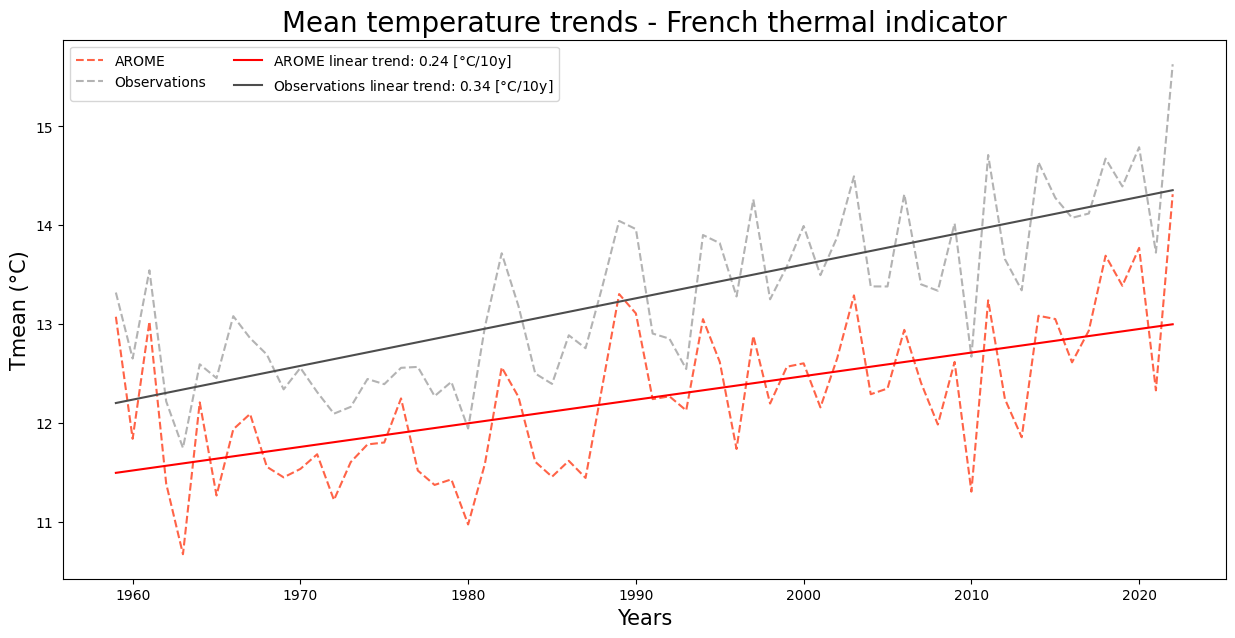
\includegraphics[width=\linewidth]{fig8.png}
  \caption{\DIFaddFL{Temporal evolution of the annual mean temperature between 1959 and 2022. For the observations, the time-series are computed from the French thermal indicator, i.e. the mean of a given set of 30 stations with homogenised data, which are the reference temperature stations in France \mbox{%DIFAUXCMD
\citep{gibelin-etal-2014}}\hskip0pt%DIFAUXCMD
. For the model, the time-series are computed over the mean of the 30 grid-points that are the closest to the stations. For each time-series, the trend is computed using a linear regression.}}\label{fig:trend_tempe}
\end{center}
\end{figure}

\DIFadd{It should be noted that temperature trends (cf. Figure~\ref{fig:trend_tempe}) with the AROME model forced by ERA5 are about one-third weaker than observed trends. This implies a dampening of the Clausius-Clapeyron-related component of extreme precipitation trends, which is expected to influence the magnitude of the trends we can detect.
}

\DIFadd{The weaker simulated temperature trend suggests that either the model's sensitivity to radiative forcings or the boundary conditions provided by ERA5 lead to a dampened warming signal in France compared to observations. Since aerosols and greenhouse gases evolve realistically in this simulation (Section~2.2), the temperature trend underestimation likely stems from the model's internal sensitivity or from the driving reanalysis.
}

\subsubsection{\DIFadd{Precipitation and modeling limitations}}\label{precipitation-limitations}

\DIFaddend First, station precipitation measurements are frequently affected by undercatch errors, which are particularly pronounced in cold and mountainous regions with strong winds. \DIFdelbegin \DIFdel{They can also show heterogeneity, }\DIFdelend \DIFaddbegin \DIFadd{Because undercatch typically leads to an underestimation of actual precipitation (especially for high-intensity, short-duration convective events), correcting for these errors would increase the observed extreme values. Consequently, the model's underestimation of hourly extremes is likely even larger than what we report here. Furthermore, station time series can also exhibit some inhomogeneities (non-climatic shifts in the time series caused by changes in station location, environment, or sensor types over decades), which could introduce local artificial trend components, }\DIFaddend although the data used here have been quality-controlled by Météo-France.

Second, raingauges provide measurement over short periods, particularly the hourly data that are available since the 1990s only. This is particularly problematic when studying extremes within a GEV framework, as only one value (the maximum value) is used per year. In some cases, isolated outliers can significantly influence estimates of the return level \citep{Zeder2024}. 
For example, in Figure \ref{fig:map_hourly_trend}, some individual points stand out from their surroundings, which is probably due to sampling bias and not to differences in climate. To make the estimation more robust, other solutions include taking into account threshold exceedances within a generalized Pareto distribution (GPD) framework, or using a distribution modeling all precipitation values, such as the recent extended generalized Pareto distribution \citep{haruna-etal-2025} \DIFaddbegin \DIFadd{or the Simplified Metastasis Extreme Value (SMEV) distribution \mbox{%DIFAUXCMD
\citep{marra2020, correa2025, lompi2025}}\hskip0pt%DIFAUXCMD
}\DIFaddend , or using a neighborhood or region-of-influence approach \citep{blanchet2021explaining} to reduce sampling bias by using more data.
All these methods have their advantages and disadvantages. Our general advice is not to interpret trends at an individual point, but to look for consistent trends across regions, to avoid over-interpretation.

Third, the stations are not evenly distributed across the country. In particular, hourly stations are lacking in the Alps, the Pyrenees and, to a lesser extent, the Massif Central. This naturally has an impact on our evaluation measures (correlation and bias) and prevents us from fully evaluating AROME in mountainous regions.

Finally, a limitation of the evaluation is that it compares point-scale raingauge measurements with 2.5 km $\times$ 2.5 km AROME grid-box averages. This mismatch in spatial support is relatively modest for daily accumulations, but it becomes a major limitation at the hourly scale: a single convective core may affect only part of a grid cell, so that local station extremes can be much higher (or lower) than the corresponding AROME value even when the event is realistically simulated at the grid-box scale. A high-resolution gridded observational product would therefore be better suited to evaluating hourly extremes than individual stations. In this respect, Météo-France’s COMEPHORE product -- a 1 km, hourly radar-gauge precipitation reanalysis over metropolitan France -- would be particularly valuable \citep{MeteoFrance_COMEPHORE_dataGouv}. It would have been interesting to include COMEPHORE in this study, but the reanalyses only begin in 1997 and the method for calculating the rainfall fields changed in 2007, which could affect trend estimation.

%DIF < Finally a limitation of the comparison at hourly scale is that it is done over 1990-2022 to fit the data availability. It could be argued that 
\DIFdelbegin %DIFDELCMD < 

%DIFDELCMD < %%%
\DIFdelend Another limitation stems from the modeling framework. We have applied a non-stationary GEV framework to estimate trends in extremes. This requires more parameters to be estimated and additional assumptions to be made about the shape of the trends. Here, we have assumed that the distribution of parameters, and therefore return levels, evolve linearly over time. This is obviously a simplification, as i) there is no physical reason for the evolution to be linear, ii) there is no direct physical dependence between return levels and time. The linearity assumption could be relaxed by considering non-linear transfer functions (e.g. power functions), with the risk of over-fitting and increased uncertainty if more parameters have to be estimated. Here, as in many other studies based on GEV distributions, we prefer to use a rigid (linear) relationship to increase robustness. Previous studies analyzing the relationship between temperature and precipitation \citep{DaSilva2025} lead us to believe that temperature might be a more appropriate covariate.
However, which temperature to choose and at which scale (e.g. local temperature at the time of the event, annual region-mean temperature, sea-surface temperature)  is a matter of debate in itself \citep{Schroeer2018, Dash2023, Zeder2020}, which is why we chose to keep time as the simplest covariate. Temperature change over the recent past is anyway close to linear in time, so we believe that the magnitude of the trends would be barely affected.



\subsection{Climatology: consistencies and divergence}\label{climatology-consistencies-divergence-and-limitations}

The results confirm that AROME correctly reproduces the main rainfall
regimes over metropolitan France, as supported by the literature \citep{Fumiere2020,Caillaud2021,hess-28-2579-2024,LucasPicher2024,Cortes-Hernandez2024}. It is able to reproduce the climatological orographic intensification of precipitation over the Alps,
the Pyrenees, and the Massif Central, a pronounced transition from Atlantic to continental climatic influence in the west, and the dryness of the Mediterranean
basin. This consistency with the stations indicates a satisfactory
representation of the dynamical forcings (moisture transport by westerly
flows, orographic uplift, low-level circulation in the Mediterranean).

AROME's ability to reproduce the frequency and quantity of precipitation and the 10-year return level of daily precipitation
is maintained throughout the year. Performance declines for the
10-year return level hourly precipitation specialy in spring ($r$ = 0.38).
Studies with the previous version of the model show that AROME underestimates high-intensity precipitation (\textgreater{} 40
mm/h) \citep{Caillaud2021,poncet2024convection}. Summer
convection remains partially under-resolved despite the 2.5 km spatial
resolution. Running AROME at finer resolution might improve this, as it was shown that a 1.3 km resolution results in a better representation of maximum intensities \citep{brousseau-etal-2016}. A separate analysis (not shown) shows that
correlation increases (+30\%) for 6- and 9-hour precipitation.
One can hypothesize that AROME spreads convective precipitation too widely in time and in space over nearby grid points, giving underestimated local peak precipitation. Unfortunately this hypothesis cannot be fully evaluated given the sparse station network. 
%DIF < The 2--3
%DIF < km grid spacing of AROME is a major step forward for representing convection
%DIF < without parameterization, but it remains too coarse for applications
%DIF < sensitive to intense maxima \citep{prein2015regional}. 

\subsection{Trends in precipitation extremes: consistencies and
divergence}\label{trends-in-precipitation-extremes-consistencies-divergences-and-limitations}

\subsubsection{Daily data: confirmation of known patterns and model--observation consistencies}

The daily trends derived from Météo-France stations confirm and refine previously documented spatial structures of extreme-precipitation evolution in France. The significant increases in the Rhône Valley and the southern Alps (+5 to +30\%) are fully consistent with earlier regional analyses reporting an intensification of daily extremes in southeastern France \citep{Blanchet2018,blanchet2021explaining,Ribes2019}. The marked increases detected in northern France (locally up to +35\%) also agree with national-scale projections indicating a northward-shifted reinforcement of daily extremes under strong warming scenarios \citep{soubeyroux:hal-04991790}. The weak or non-significant trends observed across large parts of western and central France likewise corroborate the high spatial variability highlighted in the IPCC report \citep{IPCC2021}.

Overall, AROME reproduces the main spatial structures and magnitudes reasonably well when compared with the station-based climatology. The model correctly identifies regions of positive change (southern Alps, Rhône Valley, parts of northern France) and regions with weak or negative signals (western France, the Paris area), indicating an overall ability to capture the pattern of daily return-level evolution. However, AROME systematically underestimates the amplitude of the trends. This reduced magnitude is consistent with the underestimation of temperature trends in AROME that is about one-third weaker than observed trends (Figure \ref{fig:trend_tempe})\DIFdelbegin \DIFdel{, and with the smoothing inherent to 2.5~km grid-box values}\DIFdelend .

\subsubsection{Hourly data: new national-scale findings and limited model-observation consistency}

Unlike the daily scale, no national mapping of hourly 10-year return-level trends has previously been available for France. The present work therefore provides the first nationwide characterization of hourly extreme-precipitation trends, offering new insight into their spatial organisation.

%DIF < The station-based hourly trends exhibit far greater spatial heterogeneity than their daily counterparts, and both station-based and AROME-based relative trends are far larger at hourly than at daily scale (up to 150\%). Those signals could partly be linked to the shorter time period used at the hourly time step, making trends more sensible to natural variability. A separate analysis shows that using the whole AROME period at the hourly time step reduces by 2 to 3 the range of the relative trends.
\DIFdelbegin %DIFDELCMD < 

%DIFDELCMD < %%%
\DIFdelend Over 1990-2022, trend magnitudes in hourly extremes frequently reach $\pm 50\%$ and can exceed +100\%, with strong seasonal dependence. Coherent monthly signals emerge nonetheless: February trends in the Rhône Valley, March trends along the western Mediterranean arc, November increases in the eastern Mediterranean arc, and widespread June increases across most of France. These patterns, though noisier than daily trends, are robust in the sense that they are not produced by a single year (Figure \ref{ann:comparaison_trend}). This indicates the start of an emerging trend in hourly extremes even within the constraints of a relatively short observational period.

AROME reproduces part of the \DIFaddbegin \DIFadd{seasonal }\DIFaddend structure of these hourly \DIFdelbegin \DIFdel{signals -- particularly it concords in }\DIFdelend \DIFaddbegin \DIFadd{signals---concurring on }\DIFaddend the months associated with enhanced extreme \DIFdelbegin \DIFdel{activity---- but does not }\DIFdelend \DIFaddbegin \DIFadd{activity (Figure~\ref{fig:correlation_trend}a)---but fails to }\DIFaddend capture their spatial organization \DIFdelbegin \DIFdel{nor magnitude. Model-observation correlations remain low or near zero for most seasons and months, and the model substantially underestimates the amplitude of station-based trends. Even where stations show widespread enhancements (e.g.\ February, March}\DIFdelend \DIFaddbegin \DIFadd{and magnitude. The model systematically underestimates the magnitude of positive hourly GEV trends, leading to a much larger underestimation of relative trends at hourly than at daily scale (e.g., $ME = -82.2\%$ vs. $-2.8\%$ in June, see Fig.~\ref{fig:correlation_trend}a,b). Furthermore, hourly spatial correlations remain close to zero for most convective months (e.g.}\DIFaddend , \DIFdelbegin \DIFdel{June), AROME simulates much weaker and spatially inconsistent changes}\DIFdelend \DIFaddbegin \DIFadd{$r = 0.08$ in June and $r = 0.04$ in March, see Figure~\ref{fig:correlation_trend}c), reflecting shifts in the simulated convective precipitation zones, especially in mountain regions (such as the Massif Central and the Alps) where summer convective activity dominates}\DIFaddend . Part of this \DIFdelbegin \DIFdel{was expected: the }\DIFdelend trend magnitude underestimation is consistent with the \DIFdelbegin \DIFdel{strong }\DIFdelend underestimation of temperature trends in AROME \DIFdelbegin \DIFdel{. It is also partly due to the mismatch between point-scale raingauge measurements and 2.5 x 2.5 km AROME grid box averages. Inconsistencies in the trend spatial localization were also expected since AROME runs freely on the domain without data assimilation. Thus, depending on the weather situations - and particularly for the convective months - precipitation zones can be shifted. 
}\DIFdelend \DIFaddbegin \DIFadd{(Figure~\ref{fig:trend_tempe}). 
}\DIFaddend 

Overall, the hourly results highlight two major conclusions: i) the station-derived hourly trends presented in this study constitute a new contribution to the climatology of French precipitation extremes, revealing structured yet highly localized patterns; ii) AROME currently shows limited skill in representing both the magnitude and spatial heterogeneity of hourly return-level trends, even when significant signals are isolated, underscoring the challenges of simulating sub-daily extremes.

%DIF < \subsection{Effect of record length on the detection of trends}
%DIF < Daily and hourly trends are estimated over different periods (1959--2022 for daily data, 1990--2022 for hourly data), which could suggest that the weaker and noisier hourly signals merely reflect the shorter hourly record. To assess this, we performed two complementary sensitivity checks (results not shown). First, when the daily analysis is restricted to 1990--2022, the spatial organisation and the sign of the 10-year return level trends remain very similar to those obtained over 1959--2022, with only a modest reduction in amplitude. This indicates that the main daily-scale signals identified in southeastern and northern France are not an artefact of the longer daily record. Second, AROME-only hourly trends computed over the full 1959--2022 simulation period (Figures~Y--Z) remain weak and spatially incoherent compared with the daily trends, even when the longer model record is used. Together, these sensitivity tests suggest that the contrast between well-structured daily trends and much less robust hourly trends is not solely due to differences in record length, but also reflects the greater intermittency of convective extremes and the current limitations of AROME in representing their temporal evolution at the hourly scale.
\DIFdelbegin %DIFDELCMD < 

%DIFDELCMD < %%%
\DIFdelend \section{Conclusion}\label{conclusion}

This study evaluated the ability of the convection-permitting regional climate model AROME (2.5\,km), forced by ERA5 over 1959--2022, to reproduce the climatology and the recent evolution of extreme precipitation in metropolitan France, using Météo-France rain-gauge observations at daily (1959--2022) and hourly (1990--2022) time scales. Extremes were characterized using \DIFdelbegin \DIFdel{GEV models }\DIFdelend \DIFaddbegin \DIFadd{statistical GEV distributions }\DIFaddend (stationary and non-stationary), and trends were quantified through changes in 10-year return levels.

%DIF < At the climatological level, AROME reproduces the main spatial structures of precipitation over France, including the strong orographic enhancement over mountain ranges and the dry Mediterranean coastal belt. Agreement with station-based indicators is very high for precipitation frequency and annual totals, and remains high for daily 10-year return levels. Spatially coherent biases persist, with localized overestimation in some mountainous regions and underestimation in several coastal and foothill areas. At the hourly scale, the model shows a systematic negative bias in the 10-year return level and a strong degradation of spatial correlations in summer, consistent with an under-representation of intense convective peaks and with timing and localization errors that have a limited impact on daily accumulations but a strong impact on hourly diagnostics.
\DIFdelbegin %DIFDELCMD < 

%DIFDELCMD < %%%
%DIF < For daily extremes, station-based trends in 10-year return levels show structured, region-dependent signals over 1959--2022, with the most robust increases in the South-Eastern Alps and a reinforcement along the Rhône Valley, while large parts of western and central France exhibit weak or non-significant trends. AROME generally captures the large-scale sign and organization of these daily trend patterns, indicating that the simulation contains relevant information on the spatial structure of changes in daily extremes. However, trend amplitudes are usually weaker in the model than in the observations. This attenuation is consistent with the grid-box smoothing at 2.5\,km, with known biases in AROME for high-intensity precipitation, and with the reported underestimation of temperature trends in the ERA5-forced configuration, which likely reduces the thermodynamic contribution to changes in extreme precipitation.
%DIFDELCMD < 

%DIFDELCMD < %%%
%DIF < For hourly extremes, the station-based trends derived over 1990--2022 are much more heterogeneous and locally extreme than at the daily scale, reflecting both the intrinsic intermittency of convective precipitation and the limited length of hourly records. Despite this noise, the monthly analysis reveals recurrent windows of enhanced change (notably in late winter, early spring, late autumn, and June), suggesting that hourly extremes can exhibit seasonally concentrated signals rather than uniform annual changes. AROME captures part of the timing of these monthly windows but shows limited skill in reproducing the spatial organization and the magnitude of hourly return-level trends, with correlations close to zero for several seasons and months. These results highlight that, at 2.5\,km resolution, the representation of the temporal evolution of highly localized convective extremes remains challenging, and that point-to-grid representativeness issues strongly limit model--station consistency at the hourly scale.
%DIFDELCMD < 

%DIFDELCMD < %%%
\DIFdelend Overall, the AROME \DIFdelbegin \DIFdel{model provides }\DIFdelend \DIFaddbegin \DIFadd{simulations provide }\DIFaddend clear added value\DIFaddbegin \DIFadd{, relative to coarser regional climate models with parameterized convection, }\DIFaddend for the climatology and the spatial organization of daily extremes, and \DIFdelbegin \DIFdel{it }\DIFdelend \DIFaddbegin \DIFadd{they }\DIFaddend can support national-scale analyses of daily extreme-precipitation changes, provided that trend magnitudes are interpreted cautiously. In contrast, the evaluation indicates that hourly return levels and especially their trends are less well reproduced, with hourly trends almost inexistent in AROME. However our evaluation shows limitation at hourly scale due to spatial support mismatch between stations and grid points, and short observational record length of stations that prevented us from making the comparison over the full 1959--2022 simulation period. Future work should rely on high-resolution gridded reference datasets (e.g.\ radar--gauge reanalyses) to reduce representativeness errors and investigate the sensitivity of results to temporal and spatial aggregation (multi-hour maxima, intensity-duration-area-frequency curves, \cite{haruna-etal-2024}). These steps are necessary to assess the reliability of \DIFdelbegin \DIFdel{the AROME model' s }\DIFdelend \DIFaddbegin \DIFadd{CNRM-AROME simulations' }\DIFaddend representation of extremes, and to pave the way for its use in studying extremes in climate projections.

\section*{Code availability}
The source code for the ExtremePrecipit analysis is available on GitHub (\url{https://github.com/NCSdecoopman/ExtremePrecipit}) and is archived on Zenodo \citep{decoopman_zenodo_2026}. The DOI is: 10.5281/zenodo.18788767.

\section*{Data availability}
The precipitation datasets used in this study, including the AROME \DIFdelbegin \DIFdel{model }\DIFdelend \DIFaddbegin \DIFadd{simulation }\DIFaddend outputs and processed station data (totaling several hundred gigabytes), are hosted on Hugging Face at \url{https://huggingface.co/datasets/ncsdecoopman/ExtremePrecipit_sauv}. The AROME simulations will be available on the ESGF (\url{https://esgf.github.io/}) in 2026. Summary statistics and key  indicators are included in the code repository archived on Zenodo (DOI: 10.5281/zenodo.18788767).

\section*{Author contribution}
\textbf{ND}: Conceptualization, Methodology, Validation, Formal Analysis, Visualization, Writing - Original Draft, Writing - Review \& Editing. \textbf{JB}: Conceptualization, Methodology, Validation, Writing - Review \& Editing, Supervision. \textbf{AB}: Conceptualization, Methodology, Validation, Writing - Review \& Editing, Supervision. \textbf{CC}: Data Curation, Resources, Methodology, Writing - Review \& Editing

\section*{Competing interests}
The authors declare that they have no conflict of interest.

\section*{Acknowledgments}
This work is the result of N. Decoopman's Master thesis in collaboration between the Institute of Geosciences of the Environnement (IGE) and Office National des Forêts (ONF) - Service Restauration des Terrains en Montagne (RTM) de l'Isère. This study has received funding from Agence Nationale de la Recherche - France 2030 as part of the PEPR TRACCS programme under grant numbers ANR-22-EXTR-0005 and ANR-22-EXTR-0011. The study was also funded by the European Union through the HORIZON-EUROPE IMPETUS4CHANGE project. Views and opinions expressed are however those of the author(s) only and do not necessarily reflect those of the European Union. Neither the European Union nor the granting authority can be held responsible for them. We would like to thank Météo-France for providing their precipitation data as well as the decades of work and dedication invested in maintaining their observational networks. We would also like to thank Elizabeth Harader-Coustau and Mathis Chevé for fruitful discussions and for providing us the data used to produce Figure \ref{fig:trend_tempe}.

%DIF < \section*{References}\label{references}
\DIFdelbegin %DIFDELCMD < 

%DIFDELCMD < %%%
%DIF < \bibliographystyle{copernicus}
\DIFdelend \bibliography{references.bib}

%DIF < \section{Annexes}\label{annexes}
\DIFdelbegin %DIFDELCMD < 

%DIFDELCMD < %%%
%DIF < \clearpage 
\DIFdelend \appendix
%DIF <  Définit la numérotation comme LettreDeSection + Numéro (ex: A1, B1)
\DIFaddbegin \clearpage
\DIFaddend \renewcommand{\thefigure}{\thesection\arabic{figure}}

\section{10-year return level of precipitation}
\setcounter{figure}{0} 
%DIF <  Réinitialise le compteur pour l'annexe A

\begin{figure}[H]
    \centering
    \DIFdelbeginFL %DIFDELCMD < \includegraphics[width=\textwidth]{annexe1.pdf}
%DIFDELCMD <     %%%
\DIFdelendFL \DIFaddbeginFL 
\includegraphics[width=\textwidth]{figa1.pdf}
    \DIFaddendFL \caption{10-year return level of daily precipitation of the AROME \DIFdelbeginFL \DIFdelFL{model }\DIFdelendFL \DIFaddbeginFL \DIFaddFL{simulations }\DIFaddendFL (first row), Météo-France stations (second row), and the AROME--Station difference (third row), with the spatial correlation between the stations and their closest grid points ($r$), the bias ($ME$) and the number of stations compared (n). The statistics are derived from daily data from 1959 to 2022. The contour lines show the 400 and 800 m isolines. To ease visualization, colour scales are symmetrically saturated above the 99th percentile.}\label{ann:map_trend_daily}
\end{figure}

\begin{figure}[H]
    \centering
    \DIFdelbeginFL %DIFDELCMD < 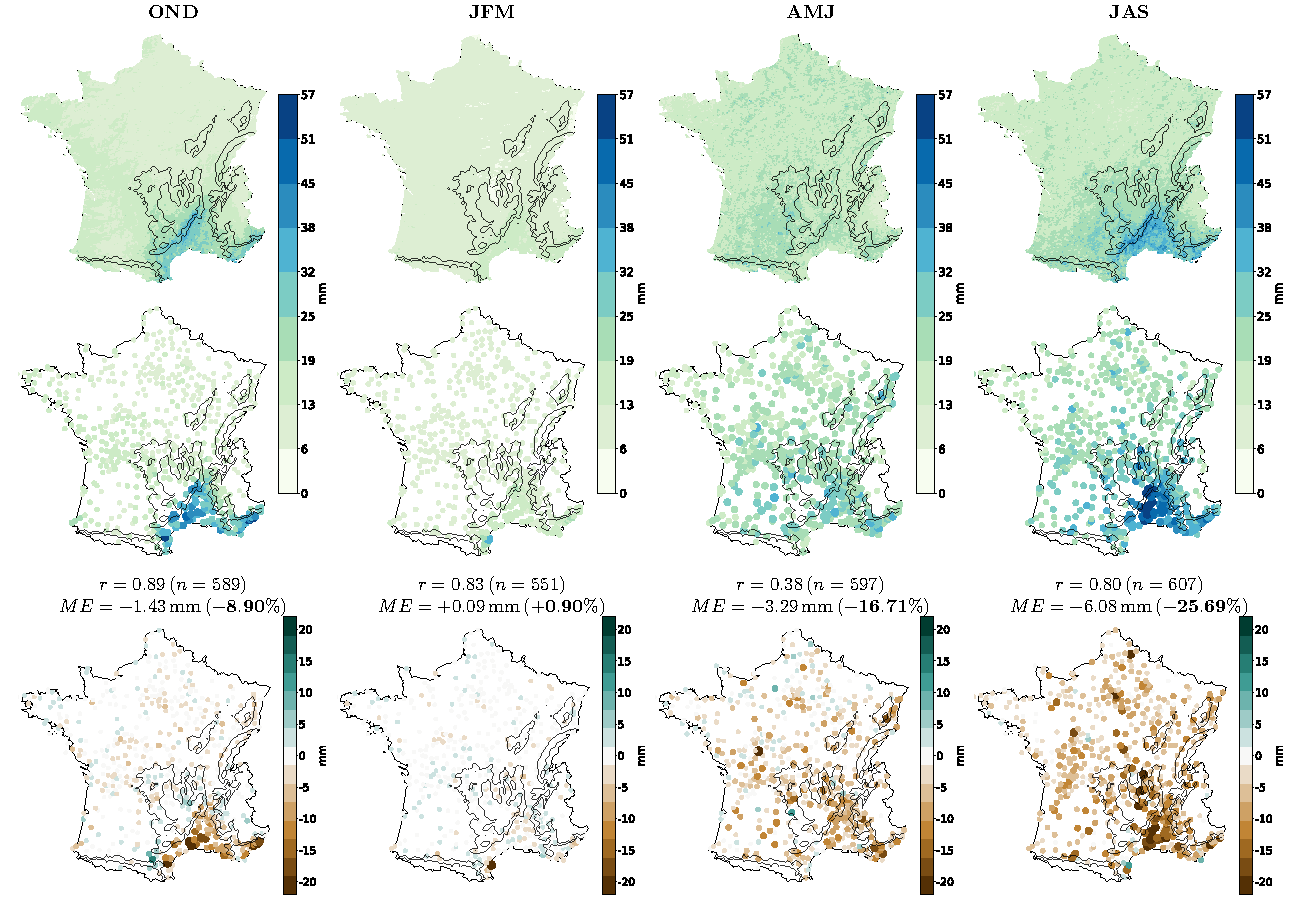
\includegraphics[width=\textwidth]{annexe2.pdf}
%DIFDELCMD <     %%%
\DIFdelendFL \DIFaddbeginFL 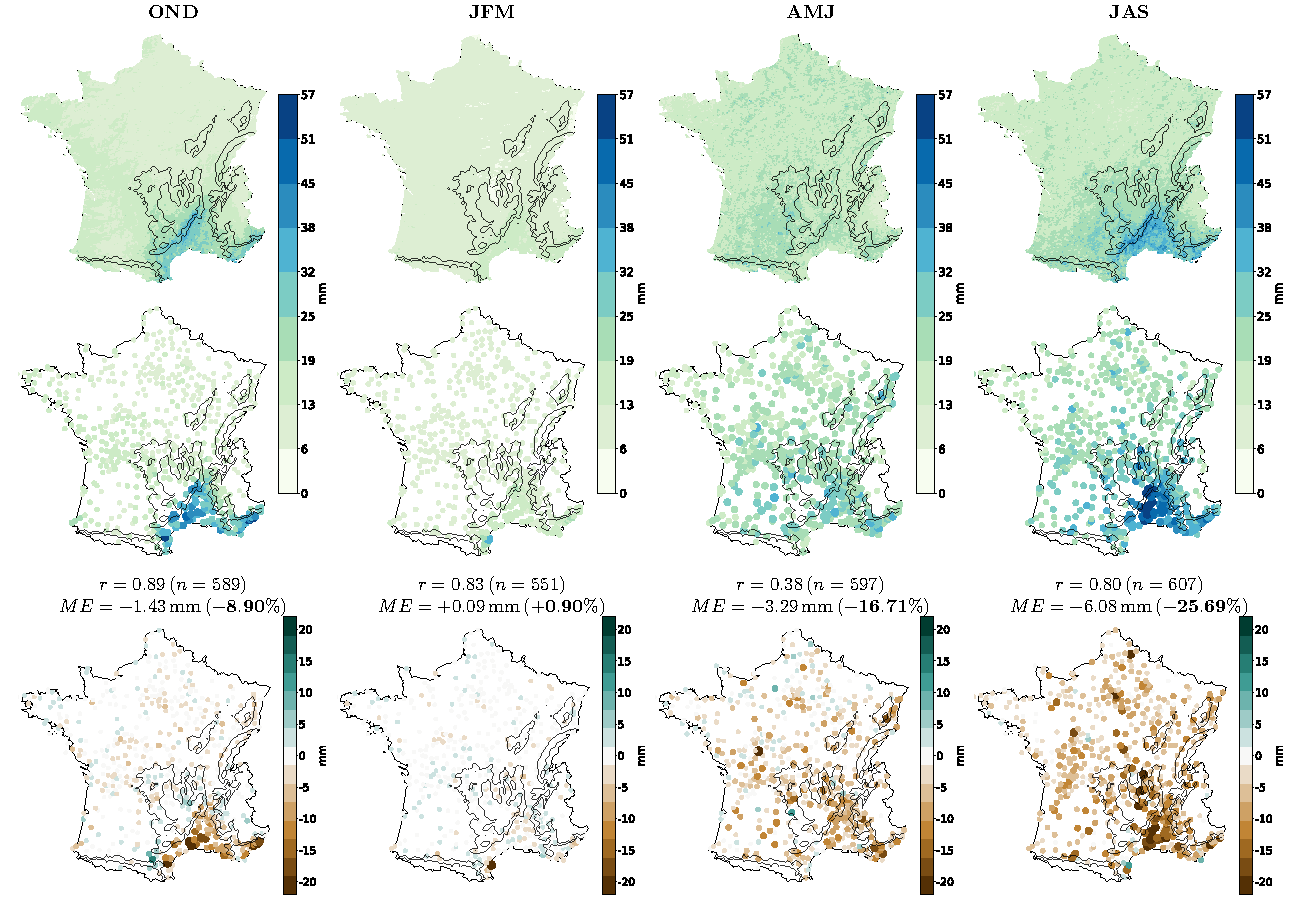
\includegraphics[width=\textwidth]{figa2.pdf}
    \DIFaddendFL \caption{10-year return level of hourly precipitation of the AROME \DIFdelbeginFL \DIFdelFL{model }\DIFdelendFL \DIFaddbeginFL \DIFaddFL{simulations }\DIFaddendFL (first row), Météo-France stations (second row), and the AROME--Station difference (third row), with the spatial correlation between the stations and their closest grid points ($r$), the bias ($ME$) and the number of stations compared (n). The statistics are derived from daily data from 1990 to 2022. The contour lines show the 400 and 800 m isolines. To ease visualization, colour scales are symmetrically saturated above the 99th percentile.}\label{ann:map_trend_hourly}
\end{figure}

%DIF < \section{Influence of a trend in GEV parameters}
%DIF < \setcounter{figure}{0} % Réinitialise le compteur pour l'annexe B (donnera Figure B1)
\DIFdelbegin %DIFDELCMD < 

%DIFDELCMD < %%%
%DIF < \begin{figure}[H]
%DIF <     \centering
%DIF <     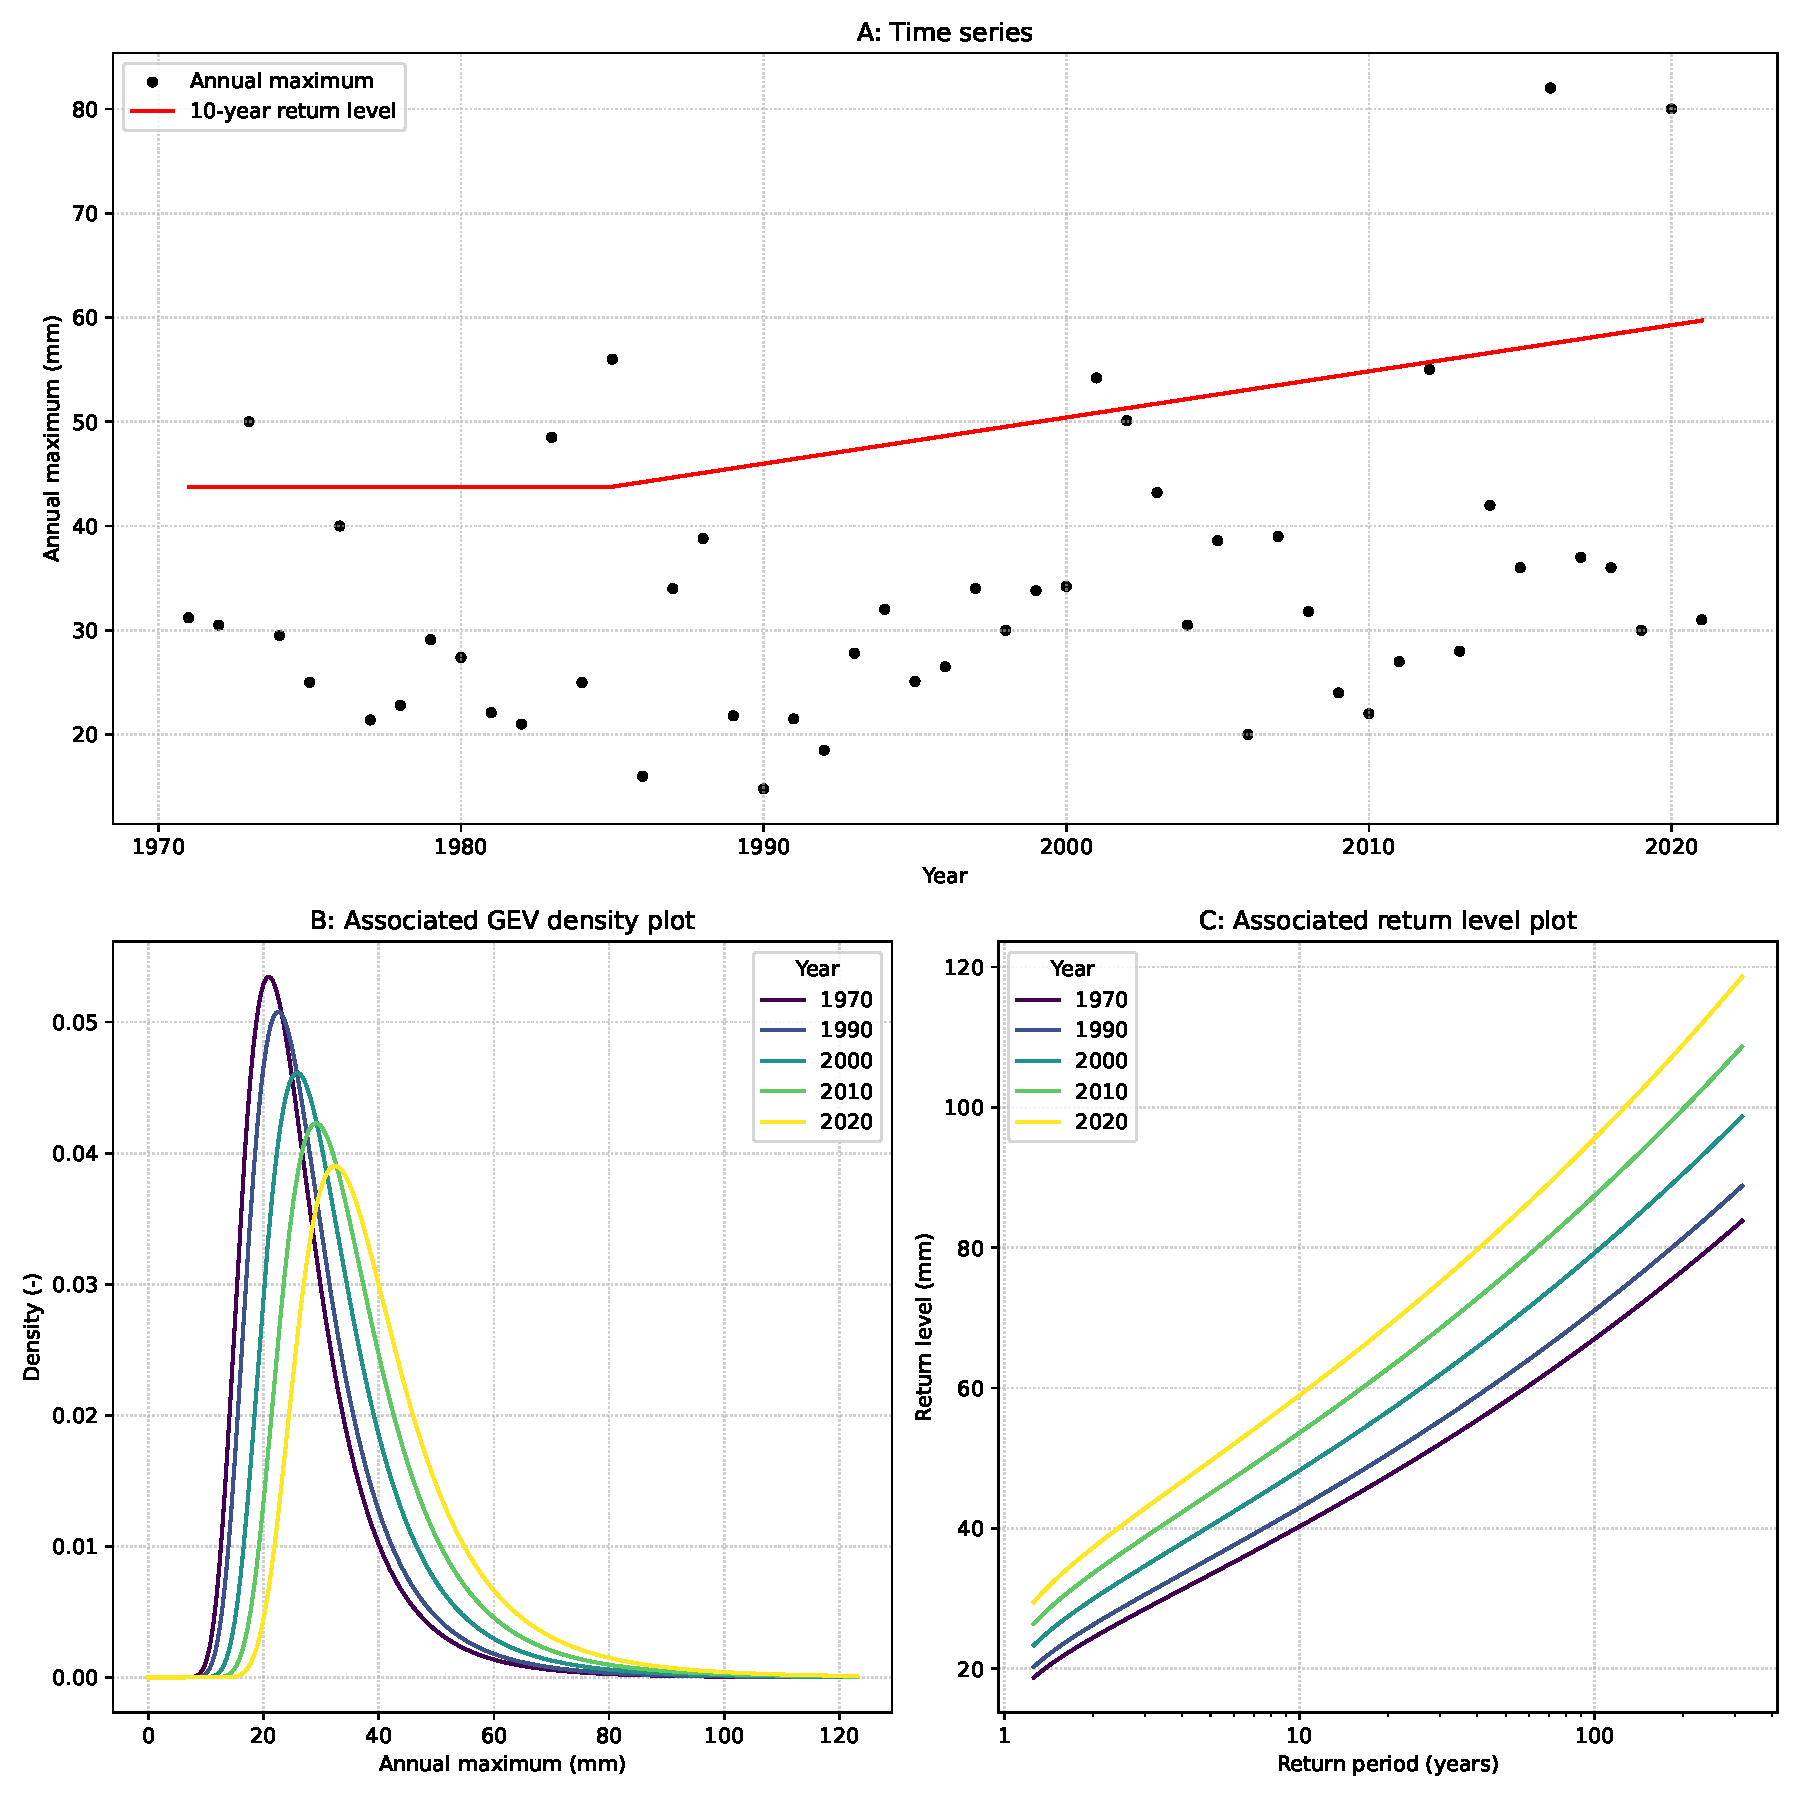
\includegraphics[width=\textwidth]{annexe3.pdf}
%DIF <     \caption{Influence of a trend in the $\mu$ and $\sigma$ parameters for a time series of annual maxima (Example: Station 45330001 located at 48.09$^\circ$ N, 1.94$^\circ$ E). (a) Time series (black dots) with the 10-year return level (red line); (b) GEV densities for selected years between 1970 (purple) and 2020 (yellow); (c) Associated return level curves.}
%DIF < \end{figure}
%DIFDELCMD < 

%DIFDELCMD < %%%
\DIFdelend \DIFaddbegin \clearpage
\DIFaddend \section{Robustness of trends when discarding the overall maxima}

\begin{figure}[htp]
\centering
    \DIFdelbeginFL %DIFDELCMD < 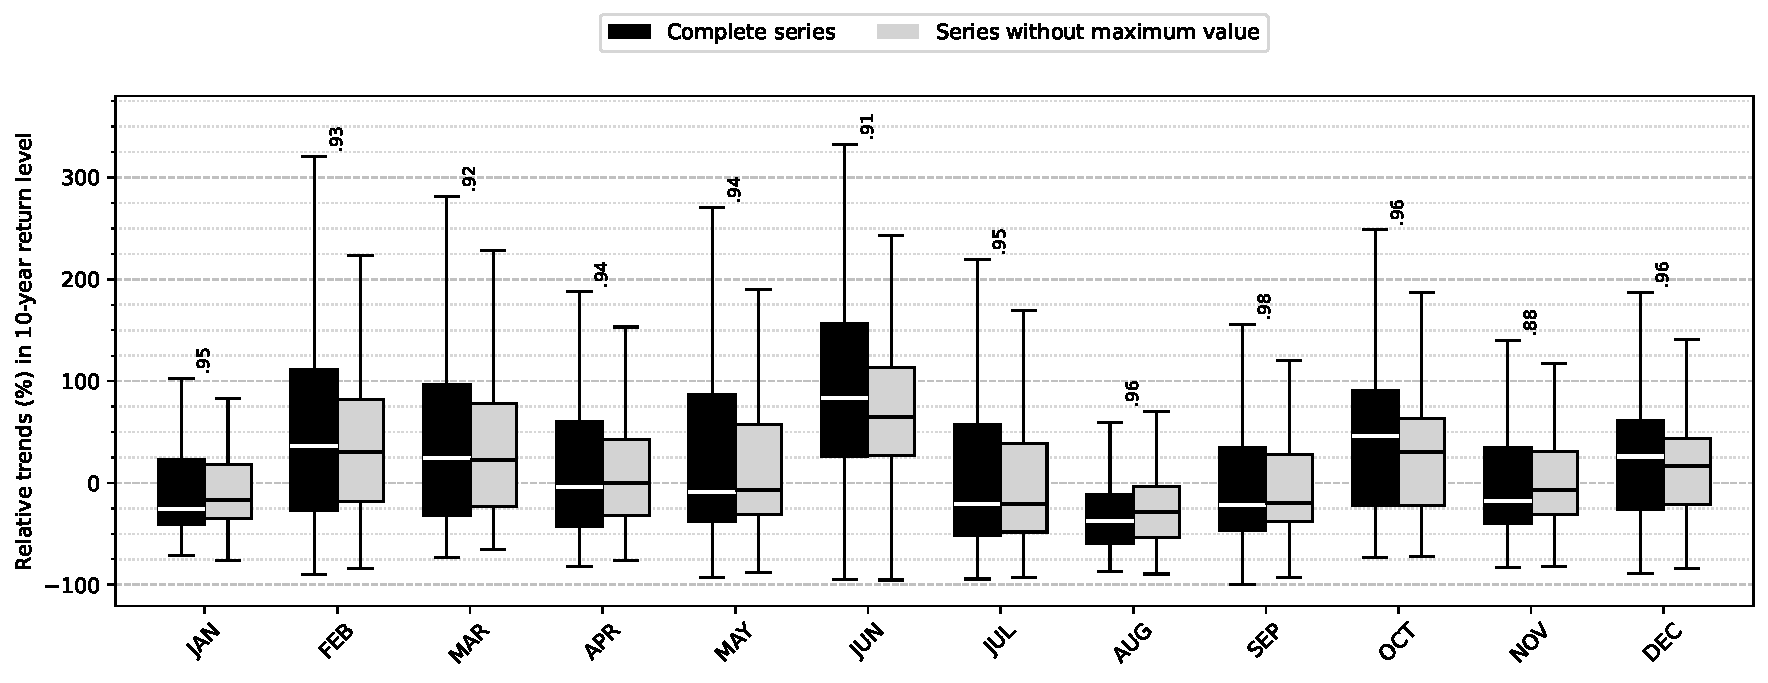
\includegraphics[width=\textwidth]{fig9.pdf}
%DIFDELCMD <     %%%
%DIF < \captionsetup{type=figure}
    %DIF < \setcounter{figure}{9}% prochaine légende = Figure 9
    \DIFdelendFL \DIFaddbeginFL 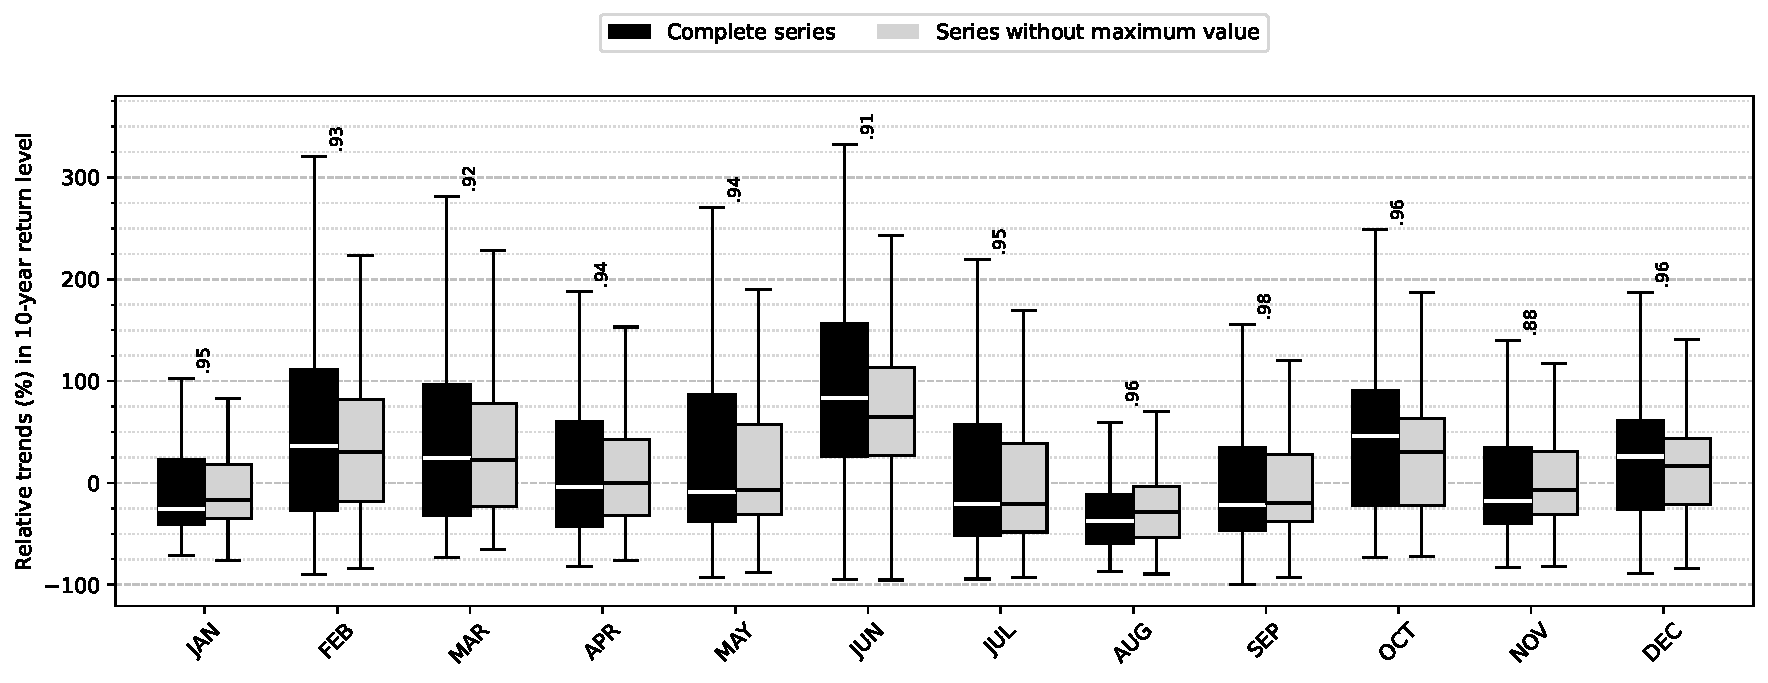
\includegraphics[width=\textwidth]{figb1.pdf}
    \DIFaddendFL \caption{Relative trends over the last thirty years ending in 2022 (\%) in the 10-year return level of hourly precipitation for Météo-France stations when considering the complete series (left) and when discarding the overall maximum (right). Only the the stations with significant trends (for the complete series) are used. The numbers written above each month indicate the Pearson correlation (r) between trends of the complete series and trends of the series without the overall maximum.}\label{ann:comparaison_trend}
\DIFaddbeginFL \end{figure}

\clearpage
\section{\DIFadd{Monthly trend maps of hourly extremes}}
\setcounter{figure}{0}

\begin{figure}[H]
    \centering
    
\includegraphics[width=0.7\textwidth]{figc1.pdf}
    \caption{\DIFaddFL{Relative monthly trends over 1990--2022 (\%) in the 10-year return level of hourly precipitation for AROME (left) and Météo-France stations (right). Display conventions: non-significant stations as open circles (white fill); significant trends close to zero as filled grey (dark outline); significant non-zero trends coloured on the map scale (uniform marker size); non-significant AROME grid cells not displayed. Metrics ($r$, $n$, $ME$) are computed on significant trends only.}}\label{ann:monthly_trend_maps}
\DIFaddendFL \end{figure}

\noappendix    
\clearpage

\end{document}